\documentclass{article}
\usepackage[utf8]{inputenc}
\usepackage[greek,english]{babel}
\usepackage{alphabeta}
\usepackage{graphicx}
\usepackage{hyperref} 
\usepackage{listings}
\usepackage{subcaption}
\usepackage{mathtools}
\usepackage{tikz}
\usepackage{multirow}
\date{}

















\begin{document}

\begin{titlepage} % Suppresses displaying the page number on the title page and the subsequent page counts as page 1
	
	\raggedleft % Right align the title page
	
	\rule{1pt}{\textheight} % Vertical line
	\hspace{0.05\textwidth} % Whitespace between the vertical line and title page text
	\parbox[b]{0.75\textwidth}{ % Paragraph box for holding the title page text, adjust the width to move the title page left or right on the page
		
		{\Huge\bfseries Τεχνικές \\ \\
		Βελτιστοποίησης\\ \\ }\\[2\baselineskip] % Title
		{\large\textit{ }}\\[4\baselineskip] % Subtitle or further description
		{\Large\textsc{Ιωάννης-Παναγιώτης \\Μπουντουρίδης}} %
	\\	\\{\large\textsc{ΑΕΜ: 8872}} % Author name, lower case for consistent small caps
		
		\vspace{0.5\textheight} % Whitespace between the title block and the publisher
		
		{\noindent \textit{work 2}}\\[\baselineskip] % Publisher and logo
	}

\end{titlepage}
\newpage
   
\section*{Θέμα 1 }

Γραφική παράσταση της συνάρτησης 
\begin{equation*}
f(x,y) = x^3 \cdot e^{-x^2-y^4}
\end{equation*}
\begin{figure*}[h!]	
     \centering  
     \advance\leftskip-0.2cm  
  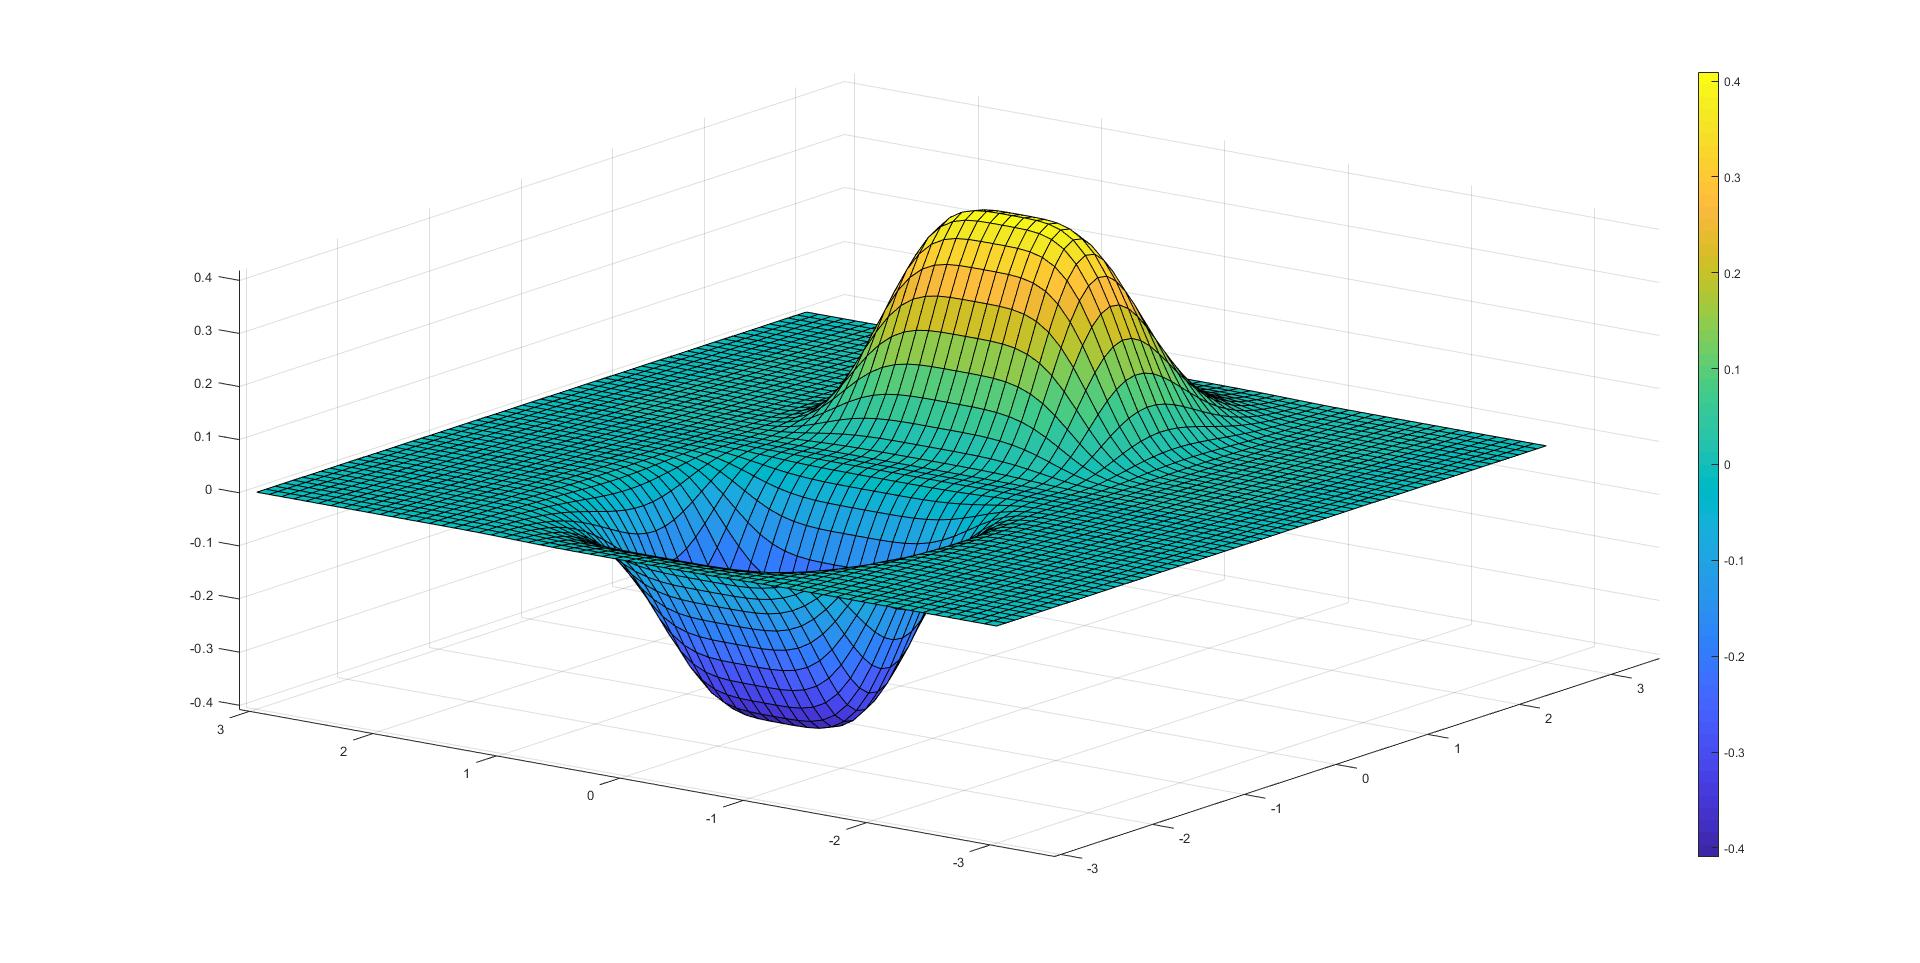
\includegraphics[width=130mm,scale=2]{functionF.jpg}
\end{figure*} 

Γραφική παράσταση της συνάρτησης 
\begin{equation*}
g(x,y) = x^4 + y^2 - 0.2sin(2πx) - 0.3cos(2πy)
\end{equation*}
\begin{figure*}[h!]	
     \centering  
     \advance\leftskip-0.2cm  
  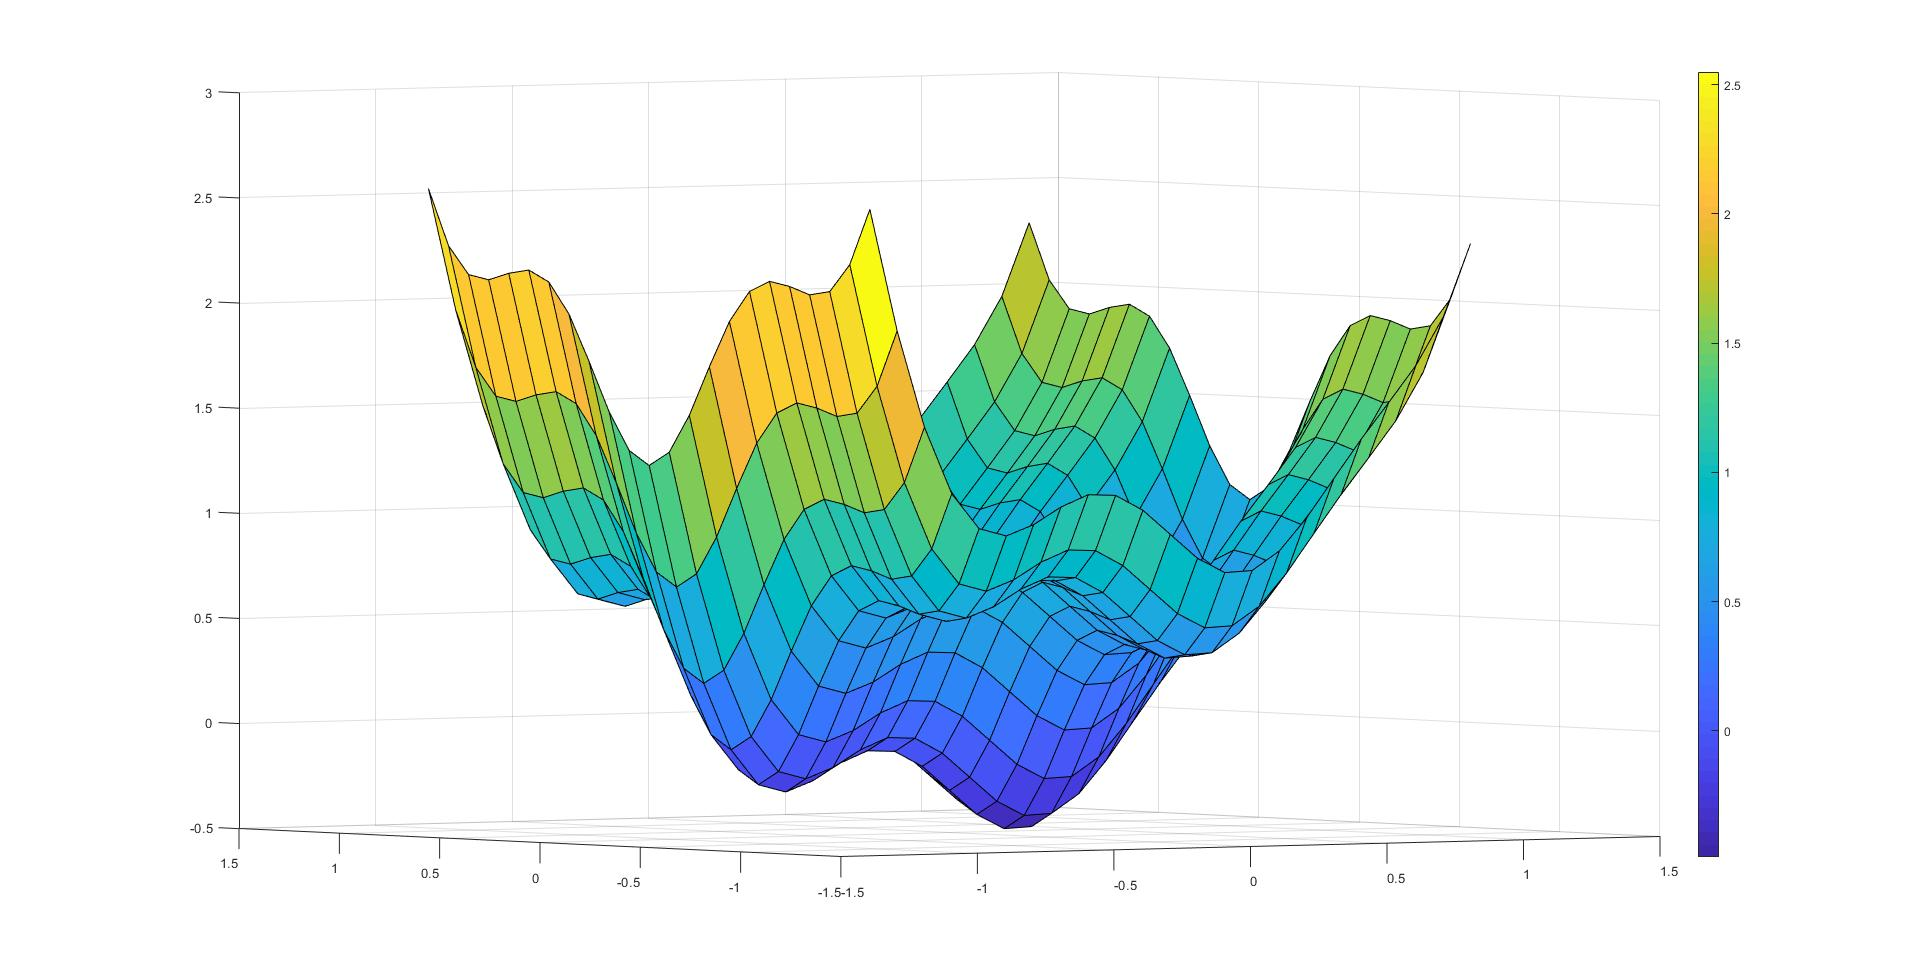
\includegraphics[width=130mm,scale=2]{functionG.jpg}
\end{figure*} 

\textit{o κώδικας των γραφικών παραστάσεων υπάρχει στο αρχείο \textbf{plot\_functions.m}}
\clearpage
\section*{Θέμα 2}
\subsection*{Ζητούμενα}
Στο πρώτο θέμα μας ζητείται να υλοποιήσουμε και να εφαρμόσουμε τη μέθοδο μέγιστης καθόδου (steepest descent) για να ελαχιστοποιήσουμε την συναρτηαη f παίρνοντας τα αρχικά σημεία i) (0,0), ii) (-1,-1), iii) (1,1).\\Το βήμα $γ_κ$ θα επιλεγεί:
\begin{itemize}
\item σταθερό της επιλογής μας
\item μεταβλητό τέτοιο ώστε σε κάθε επανάληψη να ελαχιστοποιείται η $f(x_k+g_k \cdot d_k )$ 
\item  βάσει του κανόνα Armijo
\end{itemize}
\subsection*{Περιγραφή αλγορίθμου}
Θεωρούμε το πρόβλημα ελαχιστοποίησης μιας συνάρτησης τουλάχιστον δυο φορές παραγωγίσιμης f, στην ιδέα της επαναληπτικής διαδικασίας η οποία έχει ως εξής:\\
Ξεκινάμε από το σημείο $x_0$ και παράγουμε διαδοχικά τα διανύσματα $x_1,x_2,..$ ώστε
\begin{equation*}
f(x_{k+1}) < f(x_k) \enspace k=0,1,2,...
\end{equation*} 
Ο αλγόριθμος υλοποιεί την ιδέα της επαναληπτικής καθόδου που μας οδηγεί σε ολοένα και βελτιωμένες τιμές της f, προς την ελαχιστοποίηση της.  

\begin{figure*}[h!]	
     \centering  
     \advance\leftskip-0.2cm  
  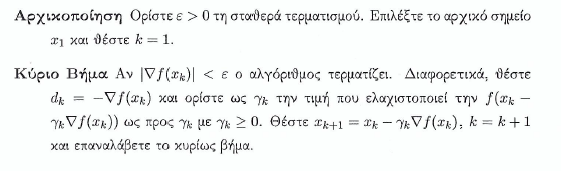
\includegraphics[width=130mm,scale=2]{desc0.png}
\end{figure*} 
\clearpage
\subsection*{Σταθερό γάμμα}
Θέτουμε ένα σταθερό $\boxed{γ_f=0.7}$ της επιλογής μας για την συνάρτηση f. Εντός του αλγορίθμου κάνουμε τους απαραίτητους ελέγχους για να δούμε αν η επιλογή μας αυτή θα συγκλίνει σε κάποιο αποτέλεσμα. Όταν η τιμή του γ είναι πολύ μικρή τότε τα βήματα των επαναλήψεων για την εύρεση ελαχίστου αυξάνουν σημαντικά. Απο την άλλη η επιλογή ενος μεγάλου γ για το σύστημα προκαλεί αστάθεια καθώς με μεγάλο βήμα ο αλγόριθμος αδυνατεί να βρει τον ελάχιστο. Επίσης για την ακρίβεια e, δηλαδή πόσο κοντά θα είμαστε στο ελάχιστο επιλέξαμε αρκούντος μικρή τιμή $\boxed{e = 10^{-4}}$\\Πιο αναλυτικά, στο ελάχιστο η παράγωγος είναι μηδέν οπότε για να προσεγγίσουμε το ελάχιστο και να βρισκόμαστε κοντά του πρέπει η παράγωγος να είναι πολύ μικρή-σχεδόν μηδέν. 
Οπότε ξεκινώντας για γάμα 0.7 έχουμε τις εξής γραφικές για την μέθοδο μέγιστης καθόδου.
\clearpage
\subsubsection*{Αρχικό σημείο (0,0) για την συνάρτηση f}
\begin{figure*}[h!]	
     \centering  
     \advance\leftskip-0.2cm  
  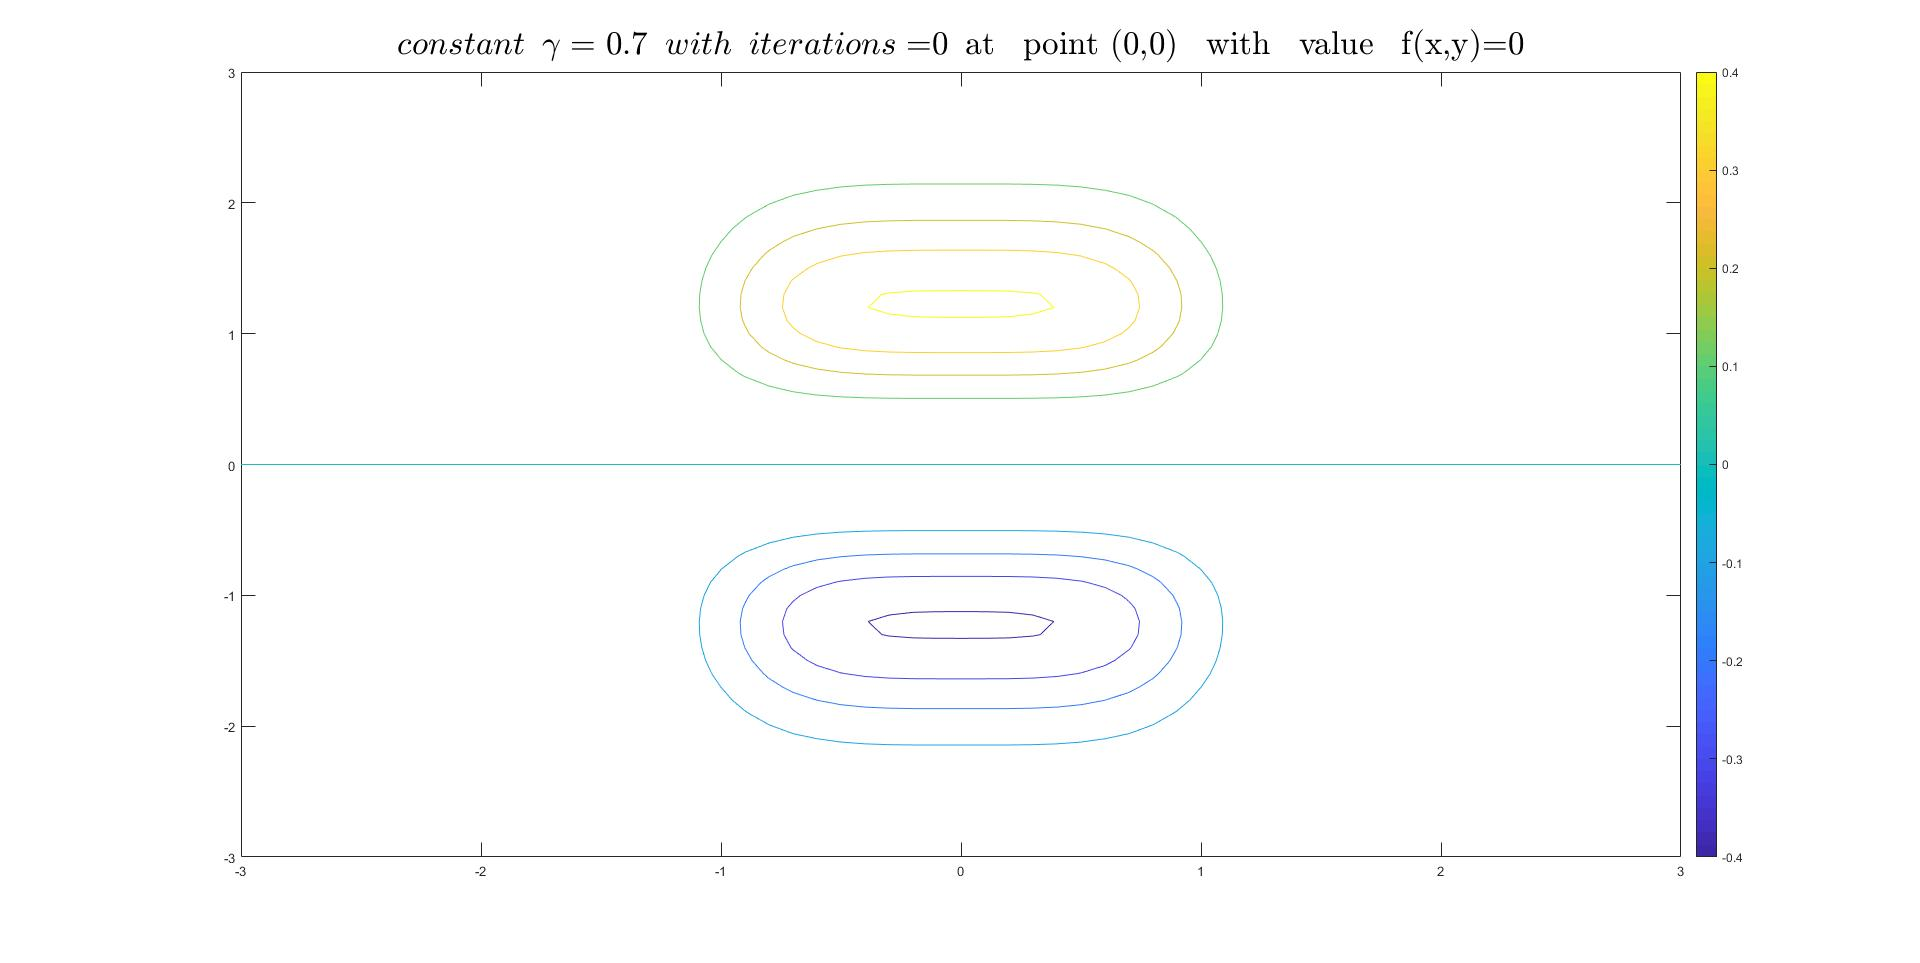
\includegraphics[width=140mm,scale=2]{t1a.jpg}
\end{figure*} 
Για αρχικό σημείο (0,0) η παράγωγος της f είναι μηδέν οπότε ο αλγόριθμος τερματίζεται πρόωρα και συνεπώς εγκλωβιζόμαστε στο σημείο f(x,y)=0.
\subsubsection*{Αρχικό σημείο (-1,-1) για την συνάρτηση f}
\begin{figure*}[h!]	
     \centering  
     \advance\leftskip-0.2cm  
  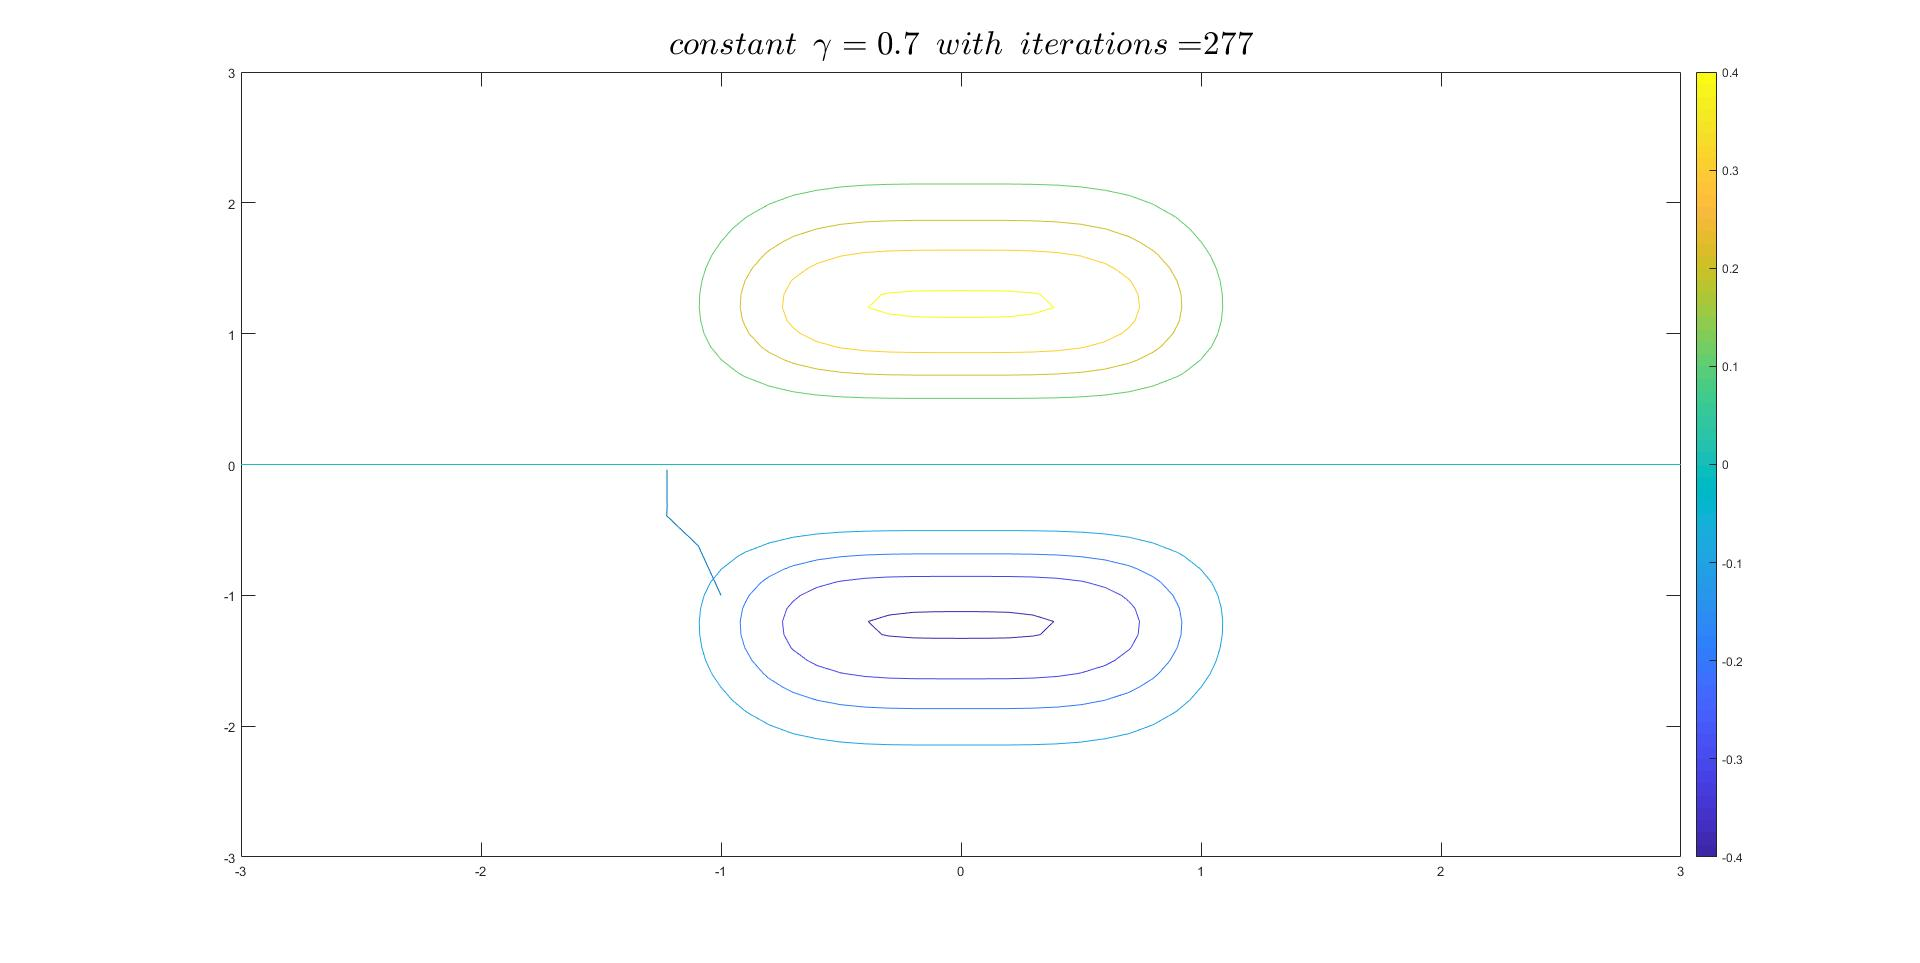
\includegraphics[width=140mm,scale=2]{t1b.jpg}
\end{figure*} 
Για αρχικό σημείο (-1,-1) μετά απο 277 επαναλήψεις καταλήγουμε στο σημείο (-1.22,-0.03) για  δοσμένη ακρίβεια e=$10^{-4}$ με τιμή f(x,y)=-0.409 που είναι  το \textbf{ολικό ελάχιστο}
\clearpage
\subsubsection*{Αρχικό σημείο (1,1) για την συνάρτηση f}
\begin{figure*}[h!]	
     \centering  
     \advance\leftskip-0.2cm  
  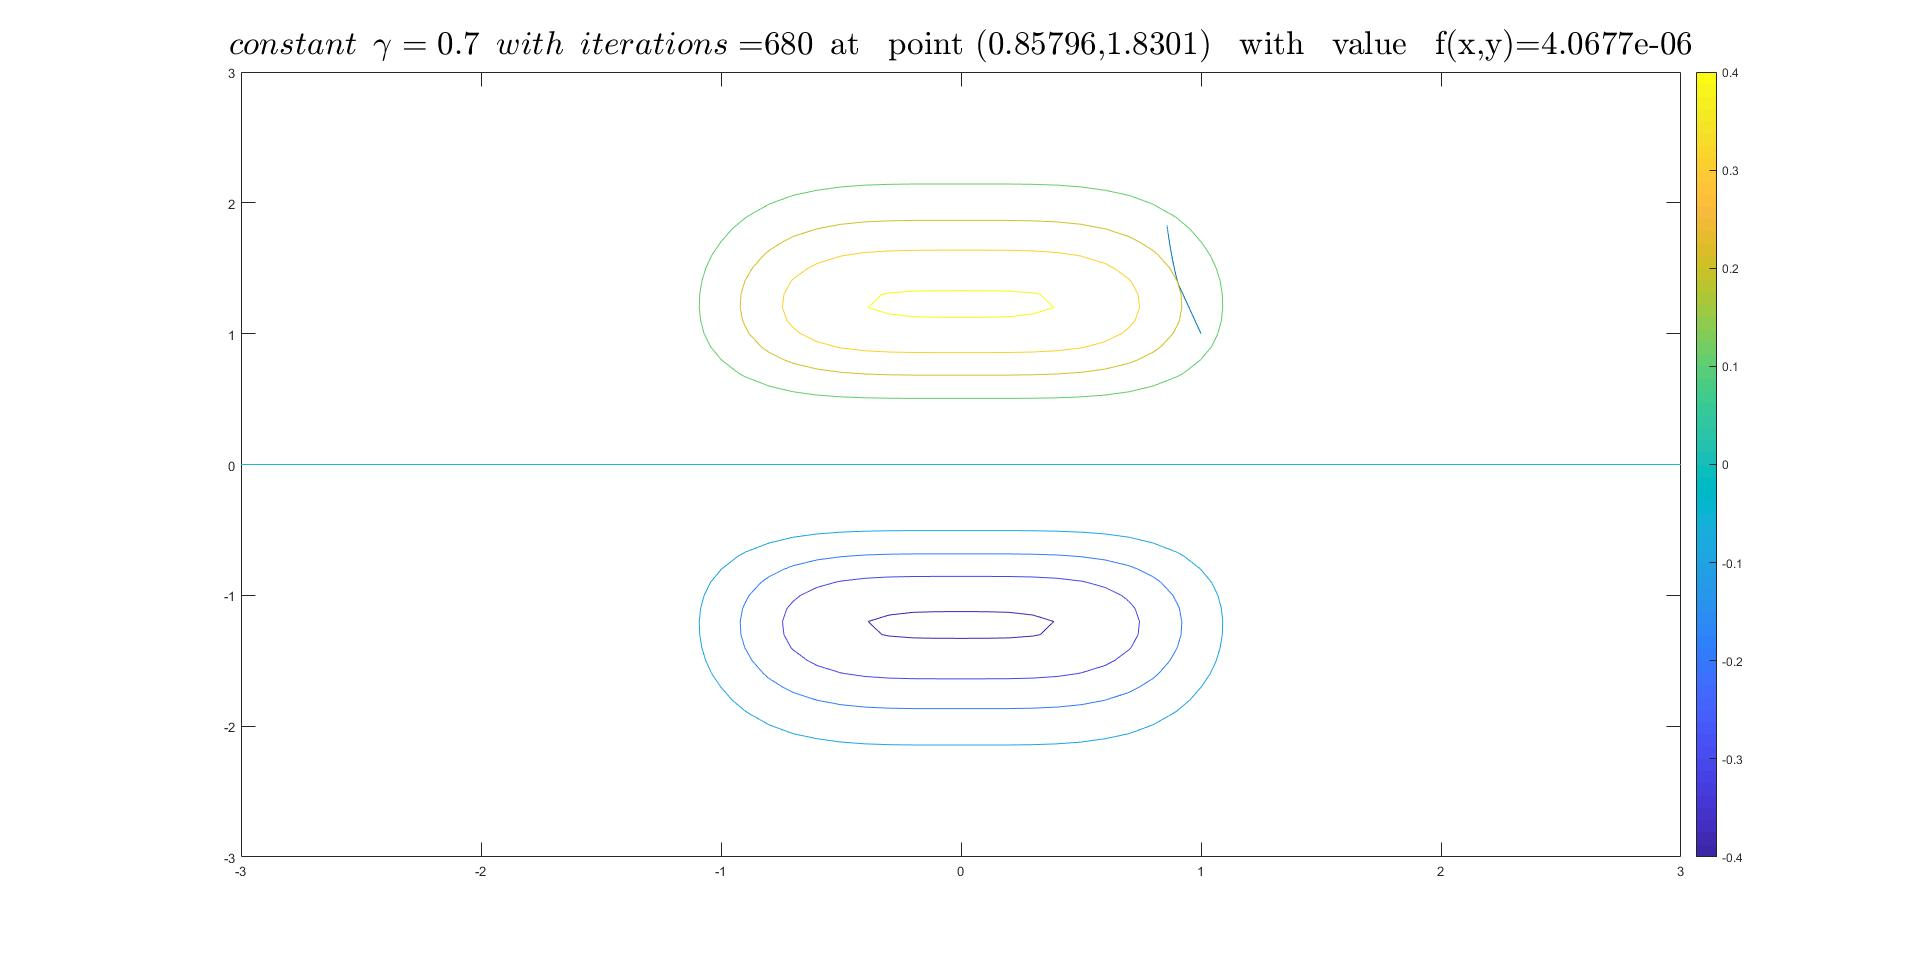
\includegraphics[width=130mm,scale=2]{t1c.jpg}
\end{figure*} 
Για αρχικό σημείο (1,1) μετά απο 680 επαναλήψεις καταλήγουμε σε τοπικό ελάχιστο (0.85,1.83) για δοσμένη ακρίβεια e=$10^{-4}$ με τιμή f(x,y)=4$\cdot 10^{-6}$. Αποτέλεσμα λογικό αφού με τόσο μικρό βήμα είναι αδύνατον να βρεθούμε στην απέναντι περιοχή του ολικού ελάχιστου χωρίς να εγκλωβιστούμε.



 

\newpage

\subsection*{Ελαχιστοποίηση $f(x_k+g_k \cdot d_k )$}
\subsubsection*{Αρχικό σημείο (0,0) για την συνάρτηση f}
\begin{figure*}[h!]	
     \centering  
     \advance\leftskip-0.2cm  
  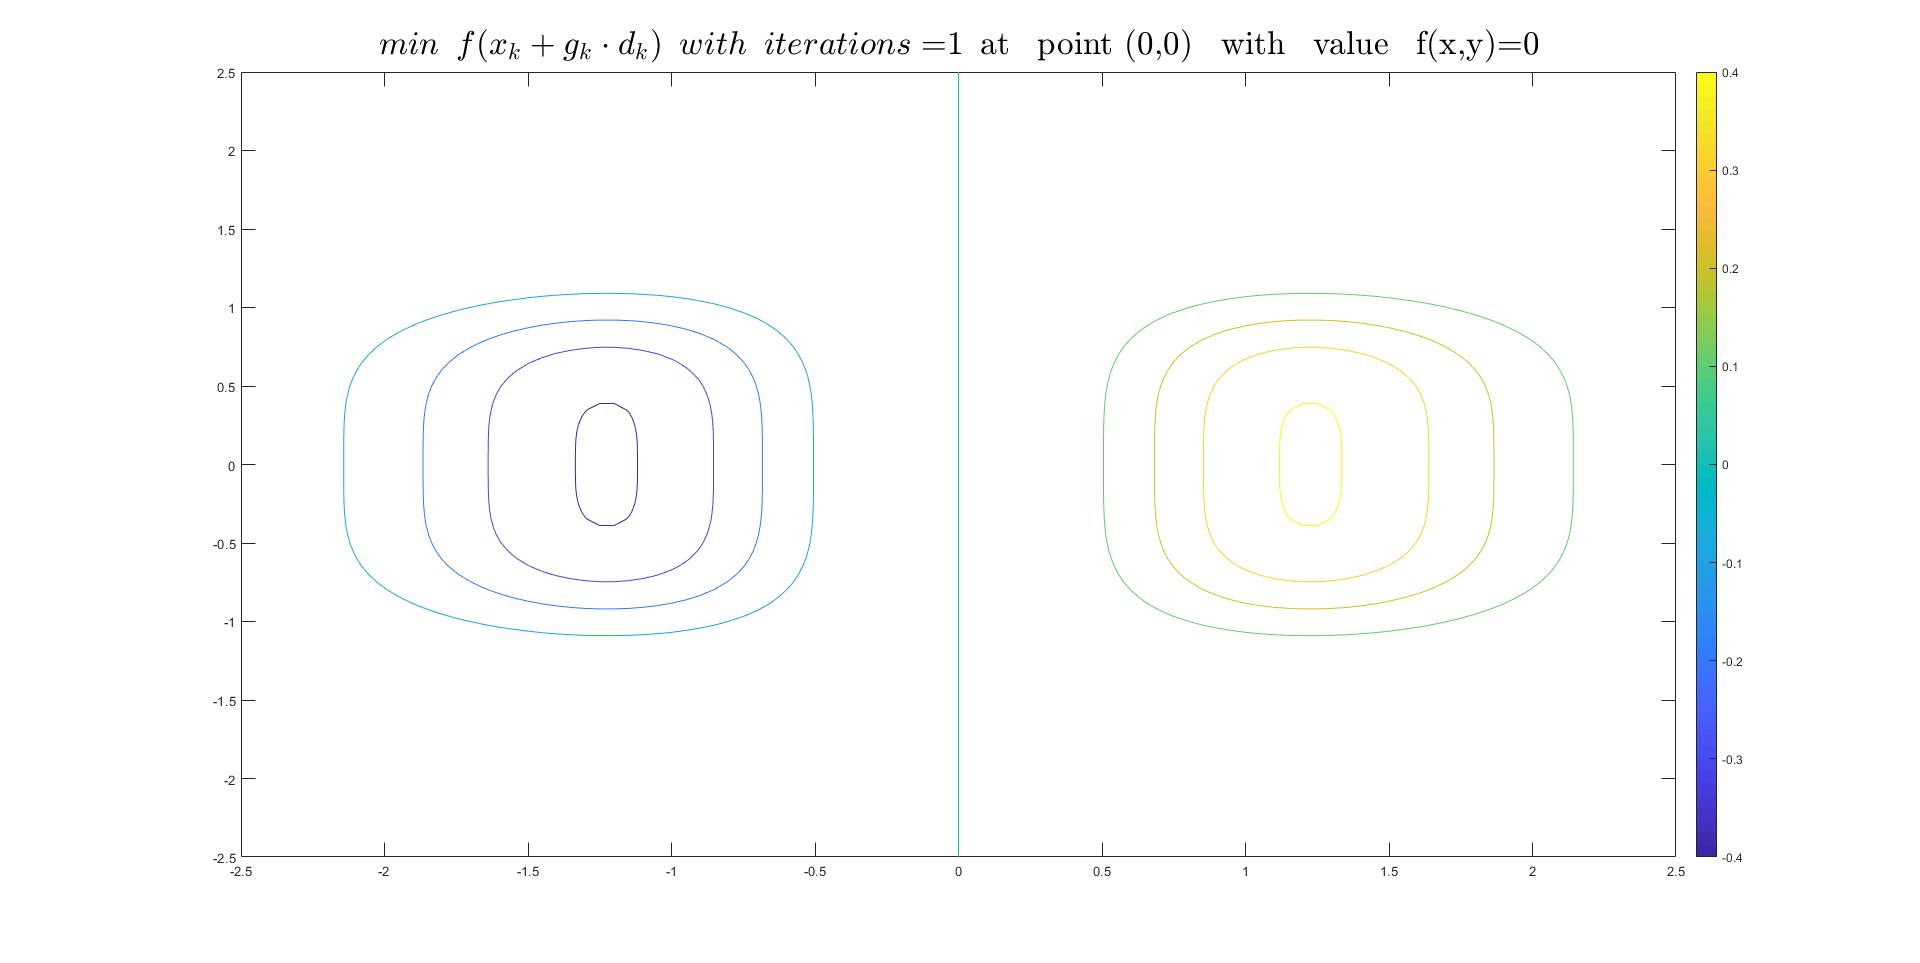
\includegraphics[width=130mm,scale=2]{mfa.jpg}
\end{figure*} 
Για αρχικό σημείο (0,0) η παράγωγος της f είναι μηδέν οπότε ο αλγόριθμος τερματίζεται πρόωρα και συνεπώς εγκλωβιζόμαστε στο σημείο f(x,y)=0.
 \subsubsection*{Αρχικό σημείο (-1,-1) για την συνάρτηση f}
\begin{figure*}[h!]	
     \centering  
     \advance\leftskip-0.2cm  
  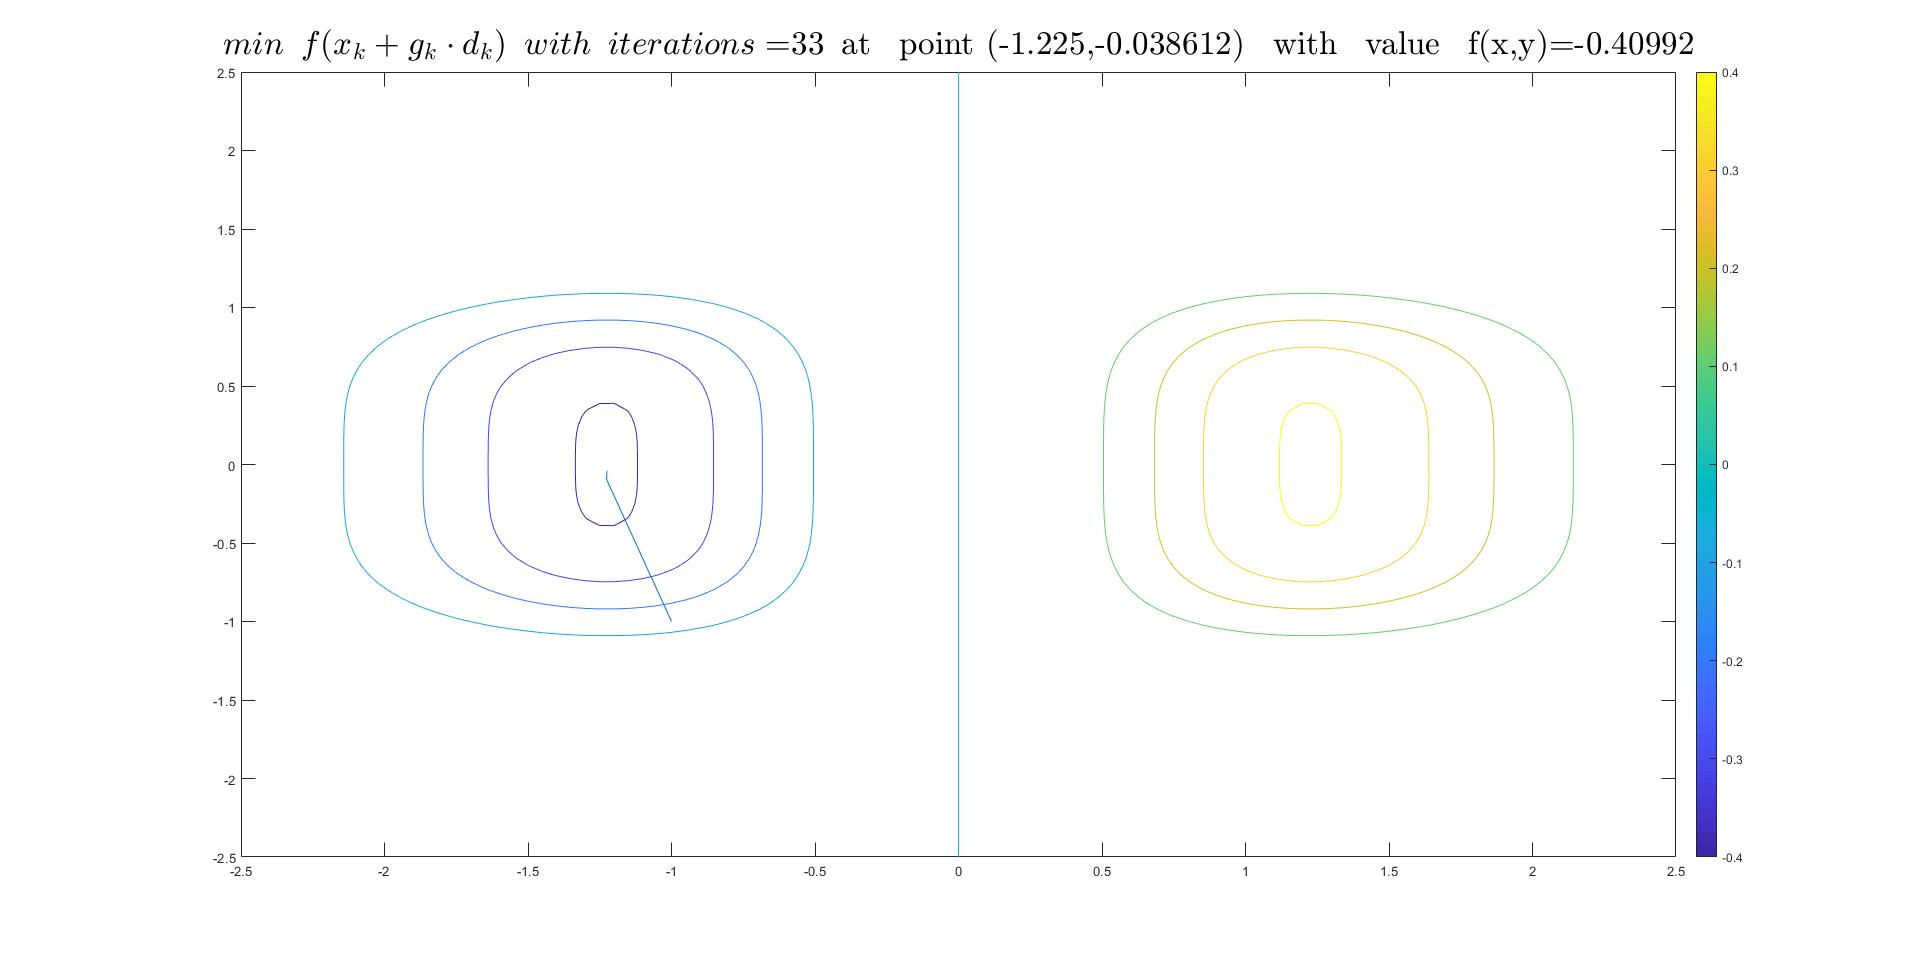
\includegraphics[width=130mm,scale=2]{mfb.jpg}
\end{figure*} 
Για αρχικό σημείο (-1,-1) μετά απο 33 επαναλήψεις καταλήγουμε στο σημείο (-1.22,-0.03) για  δοσμένη ακρίβεια e=$10^{-4}$ με τιμή f(x,y)=-0.409 που είναι  το \textbf{ολικό ελάχιστο}
\newpage
\subsubsection*{Αρχικό σημείο (1,1) για την συνάρτηση f}
\begin{figure*}[h!]	
     \centering  
     \advance\leftskip-0.2cm  
  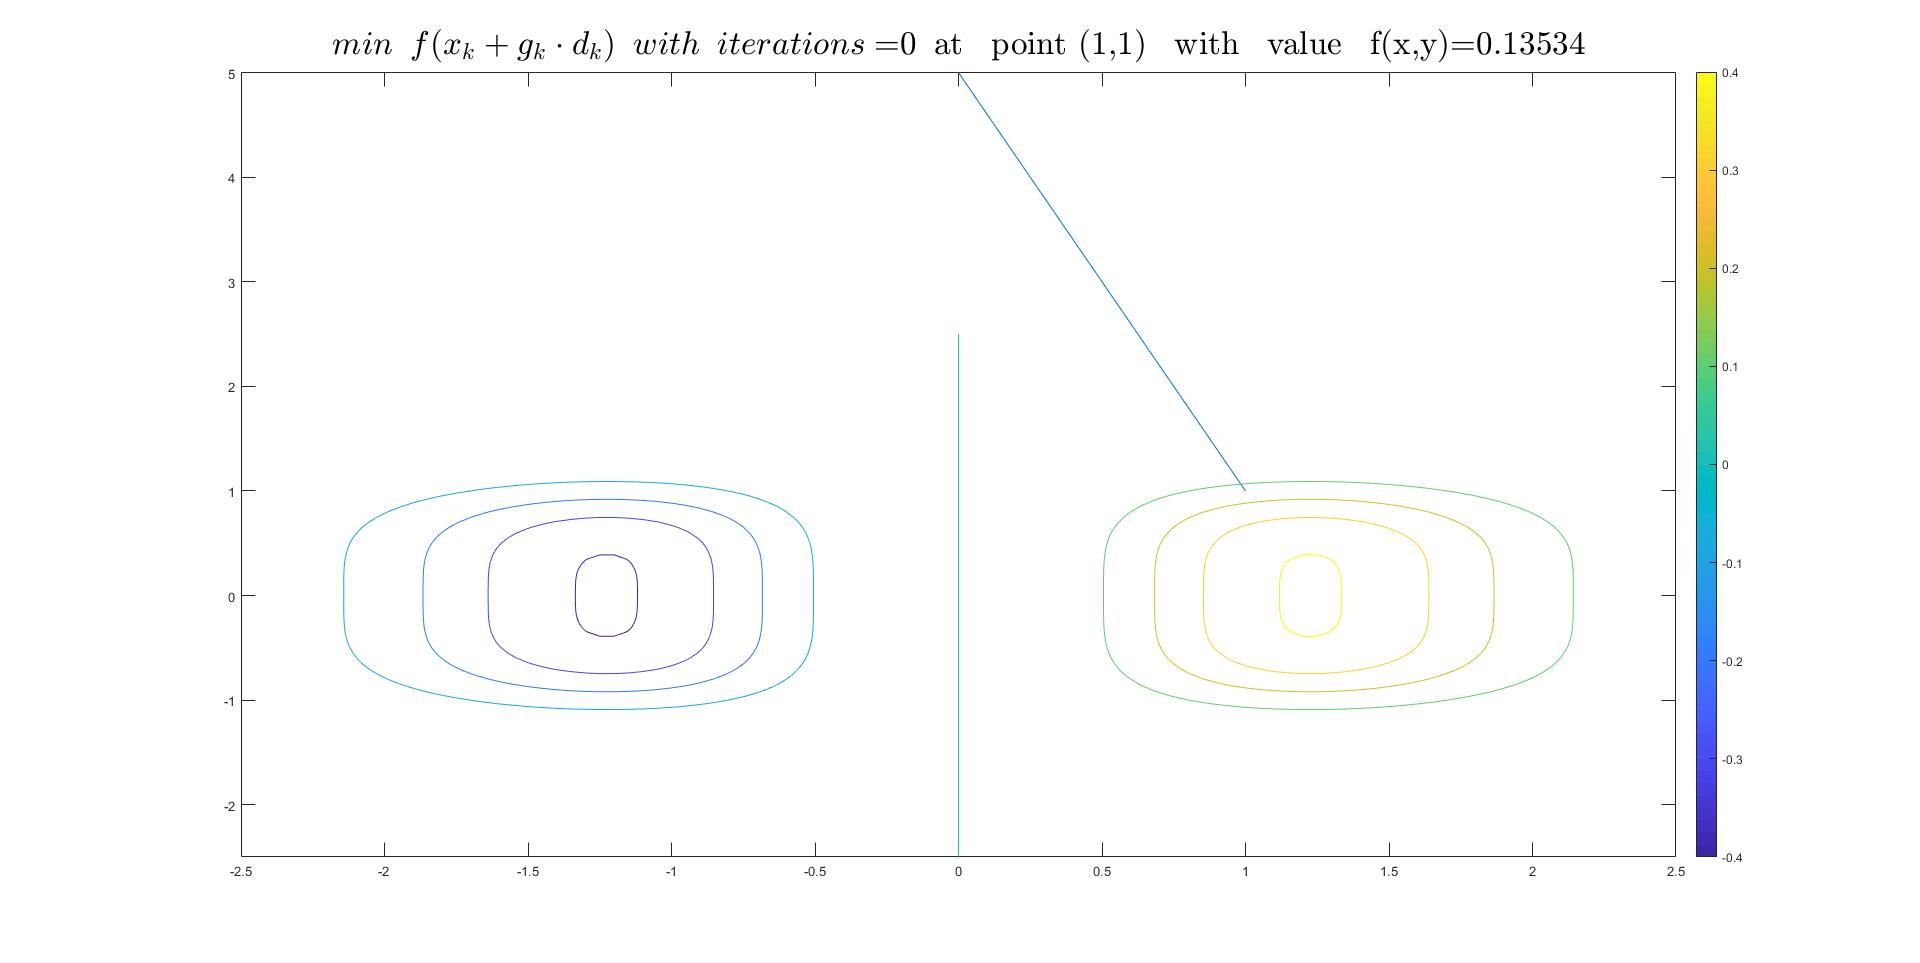
\includegraphics[width=130mm,scale=2]{mfc.jpg}
\end{figure*} 
Για αρχικό σημείο (1,1) βλέπουμε και από την παραπάνω γραφική ο αλγόριθμος  δεν συγκλίνει στο ελάχιστο. Μπορεί το γάμμα  να μην είναι σταθερό και να ακολουθεί έναν κανόνα αύξησης(όταν αυτό κρίνεται απαραίτητο ) ωστόσο ένας απλός κανόνας δεν φτάνει ώστε να καταφέρουμε την σύγκλιση του αλγορίθμου. Ο εκάστοτε κανόνας,συνήθως για να είναι αποδοτικός, πρέπει να είναι καλά σχεδιασμένος και να βασίζεται σε μαθηματικές σχέσεις και περιορισμούς. 
\clearpage
 \subsection*{Κανόνας Armijo}
\subsubsection*{Αρχικό σημείο (0,0) για την συνάρτηση f}
\begin{figure*}[h!]	
     \centering  
     \advance\leftskip-0.2cm  
  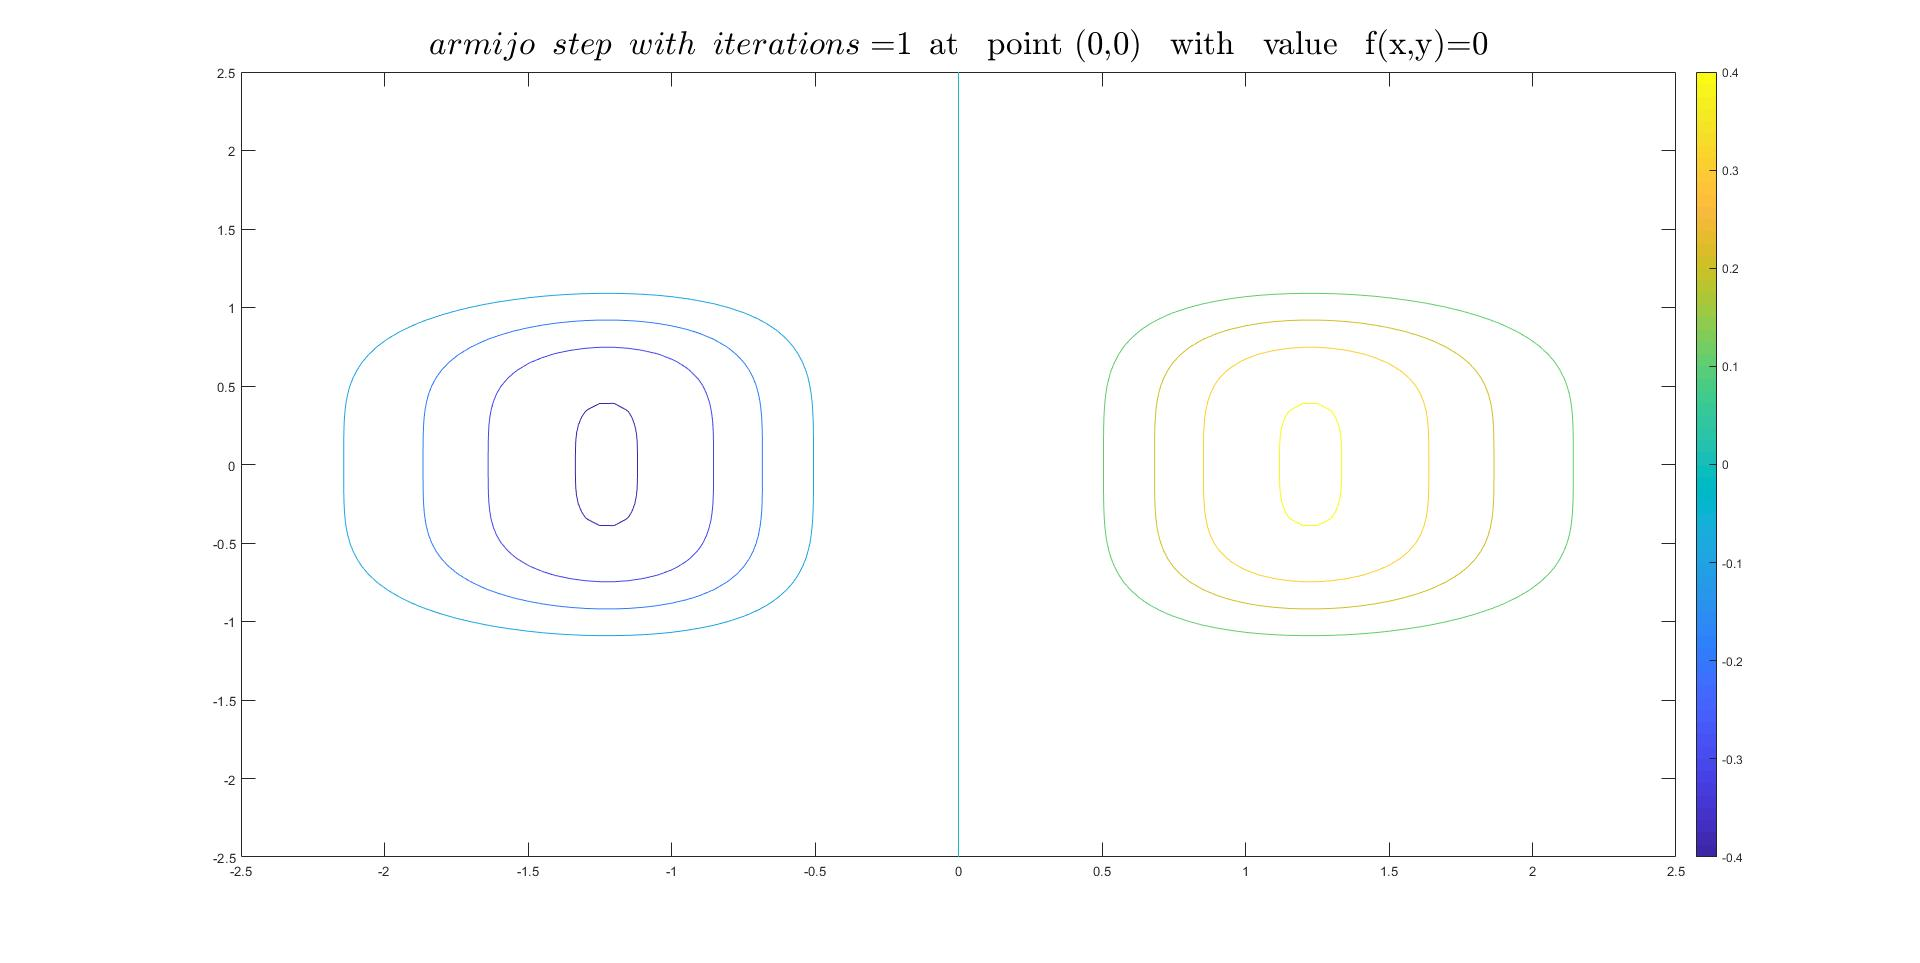
\includegraphics[width=130mm,scale=2]{arm1.jpg}
\end{figure*} 
Για αρχικό σημείο (0,0) η παράγωγος της f είναι μηδέν οπότε ο αλγόριθμος τερματίζεται πρόωρα και συνεπώς εγκλωβιζόμαστε στο σημείο f(x,y)=0.
\subsubsection*{Αρχικό σημείο (-1,-1) για την συνάρτηση f}
\begin{figure*}[h!]	
     \centering  
     \advance\leftskip-0.2cm  
  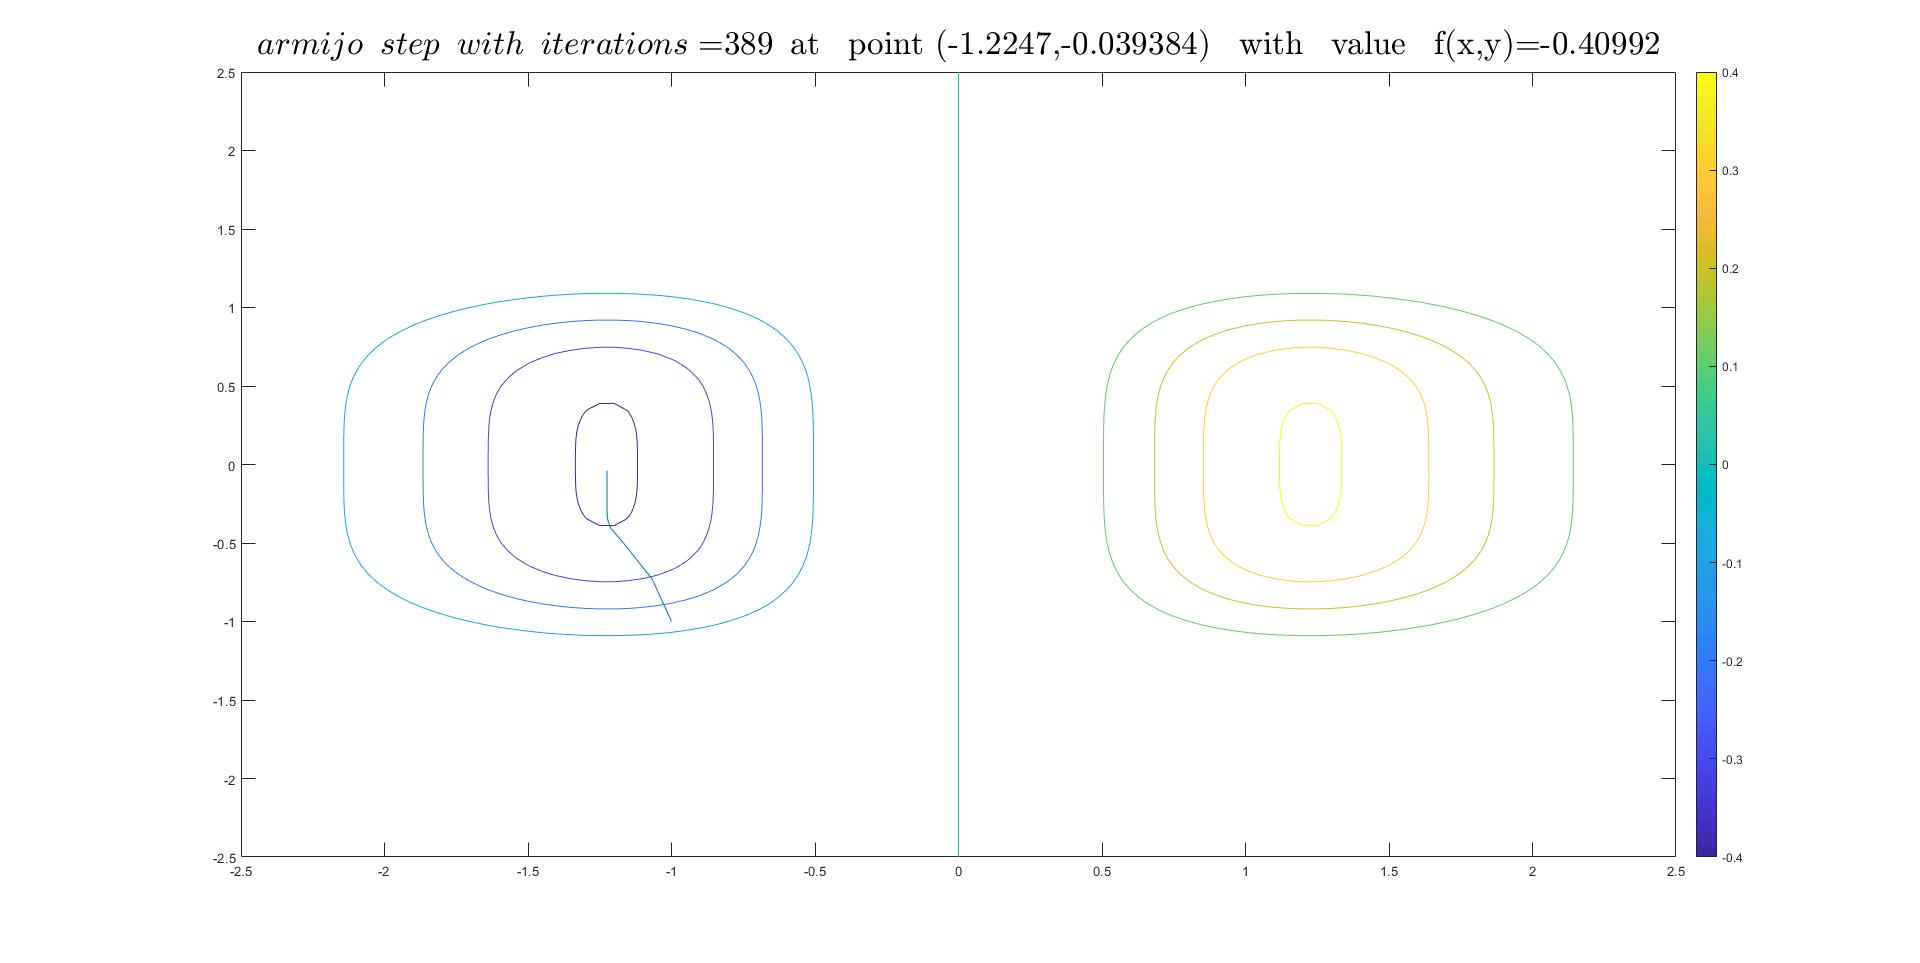
\includegraphics[width=130mm,scale=2]{arm2.jpg}
\end{figure*} 
Για αρχικό σημείο (-1,-1) μετά απο 389 επαναλήψεις καταλήγουμε στο σημείο (-1.22,-0.03) για  δοσμένη ακρίβεια e=$10^{-4}$ με τιμή f(x,y)=-0.409 που είναι  το \textbf{ολικό ελάχιστο}
\clearpage
\subsubsection*{Αρχικό σημείο (1,1) για την συνάρτηση f}
\begin{figure*}[h!]	
     \centering  
     \advance\leftskip-0.2cm  
  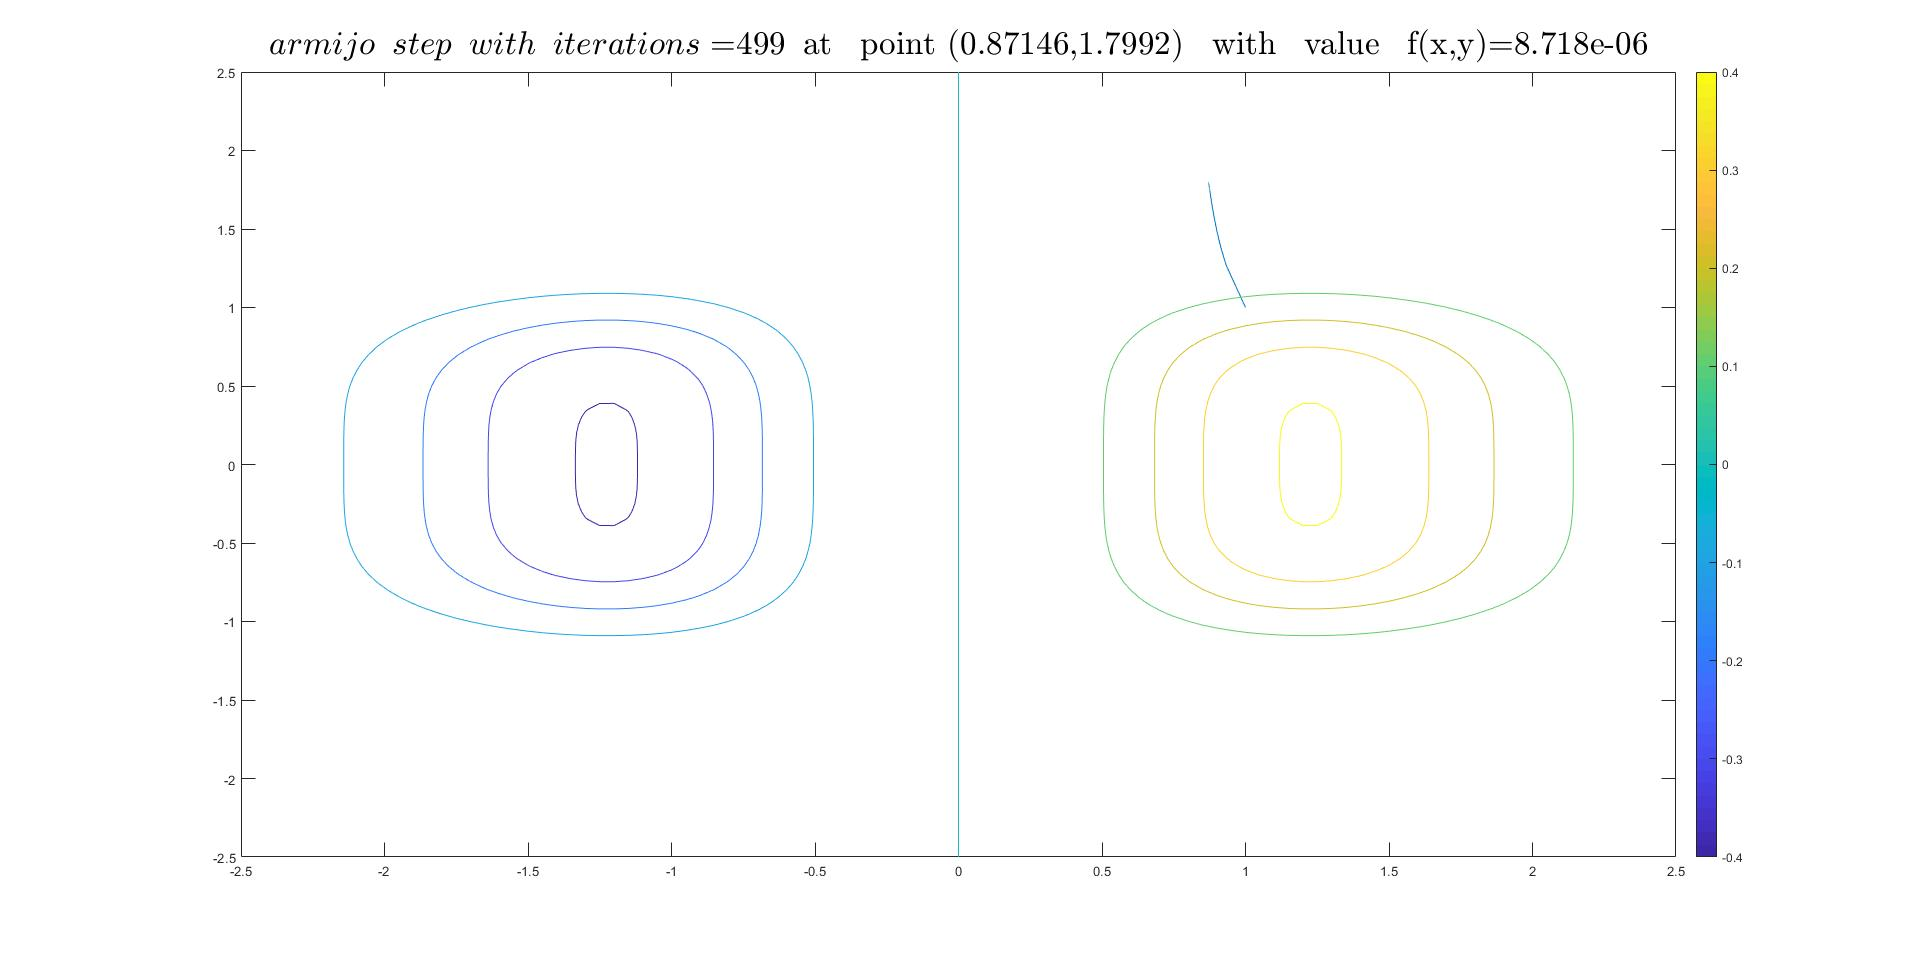
\includegraphics[width=130mm,scale=2]{arm3.jpg}
\end{figure*} 
Για αρχικό σημείο (1,1) μετά απο 499 επαναλήψεις καταλήγουμε σε τοπικό ελάχιστο (0.87,1.79) για δοσμένη ακρίβεια e=$10^{-4}$ με τιμή f(x,y)=8.7$\cdot 10^{-6}$. 
\newpage
\section*{Θέμα 3}
\subsection*{Ζητούμενα}
Στο πρώτο θέμα μας ζητείται να υλοποιήσουμε και να εφαρμόσουμε τη μέθοδο newton για να ελαχιστοποιήσουμε την συναρτηση f  παίρνοντας τα αρχικά σημεία i) (0,0), ii) (-1,-1), iii) (1,1).\\Το βήμα $γ_κ$ θα επιλεγεί:
\begin{itemize}
\item σταθερό της επιλογής μας
\item μεταβλητό τέτοιο ώστε σε κάθε επανάληψη να ελαχιστοποιείται η $f(x_k+g_k \cdot d_k )$ 
\item  βάσει του κανόνα Armijo
\end{itemize}
\subsection*{Περιγραφή αλγορίθμου}
\begin{figure*}[h!]	
     \centering  
     \advance\leftskip-0.2cm  
  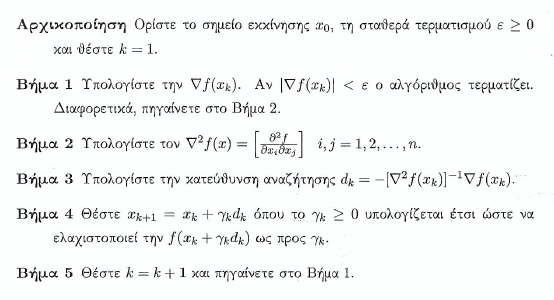
\includegraphics[width=130mm,scale=2]{desc2.png}
\end{figure*} 
\subsection*{Σταθερό γάμμα}
Θέτουμε ένα σταθερό $\boxed{γ_f=0.7}$ της επιλογής μας για την συνάρτηση f.  Όταν η τιμή του γ είναι πολύ μικρή τότε τα βήματα των επαναλήψεων για την εύρεση ελαχίστου αυξάνουν σημαντικά. Απο την άλλη η επιλογή ενος μεγάλου γ για το σύστημα προκαλεί αστάθεια καθώς με μεγάλο βήμα ο αλγόριθμος αδυνατεί να βρει τον ελάχιστο. Επίσης για την ακρίβεια e, δηλαδή πόσο κοντά θα είμαστε στο ελάχιστο επιλέξαμε αρκούντος μικρή τιμή $\boxed{e = 10^{-4}}$
\clearpage
\subsection*{Σχόλια}
Αφού υλοποιήσαμε τον αλγόριθμο της μεθόδο Newton, δοκιμάσαμε τα σημεία που μας ζητήθηκε να εξετάσουμε. Στη συνέχεια, κατασκευάσαμε τη συνάρτηση function x = checkPositiveDefinite(matrix) η οποία επιστρέφει 1 αν πίνακας πίνακας matrix είναι θετικά ορισμένος και αλλιώς μηδέν.Στα σημεία  (-1,-1) και (1,1) όπου ο αλγόριθμος τερματίζεται πριν την πρώτη επανάληψη στα  ο εσσιανός πίνακας για κάθε σημείο είναι αρνητικά ορισμένος. Οπότε όπως είναι γνωστό όταν ο εσσιανός της αντικειμενικής συναρτήσεις είναι αρνητικά ορισμένος η μέθοδος Newton είτε δεν ορίζεται είτε δίνει λύσεις πολύ μακρυά από  το σημείο του ελαχίστου για οποιοδήποτε γάμμα. Για αυτό το λόγο θα παρουσιάσουμε ενδεικτικά  την πορεία εύρεσης ελαχίστου στο σημείο  (-1,-0.5) με γάμμα σταθερό και ίσο με 0.7 και ακρίβεια .
 
\subsection*{Σταθερό γαμμα}
\subsubsection*{Αρχικό σημείο (0,0) για την συνάρτηση f}
\begin{figure*}[h!]	
     \centering  
     \advance\leftskip-0.2cm  
  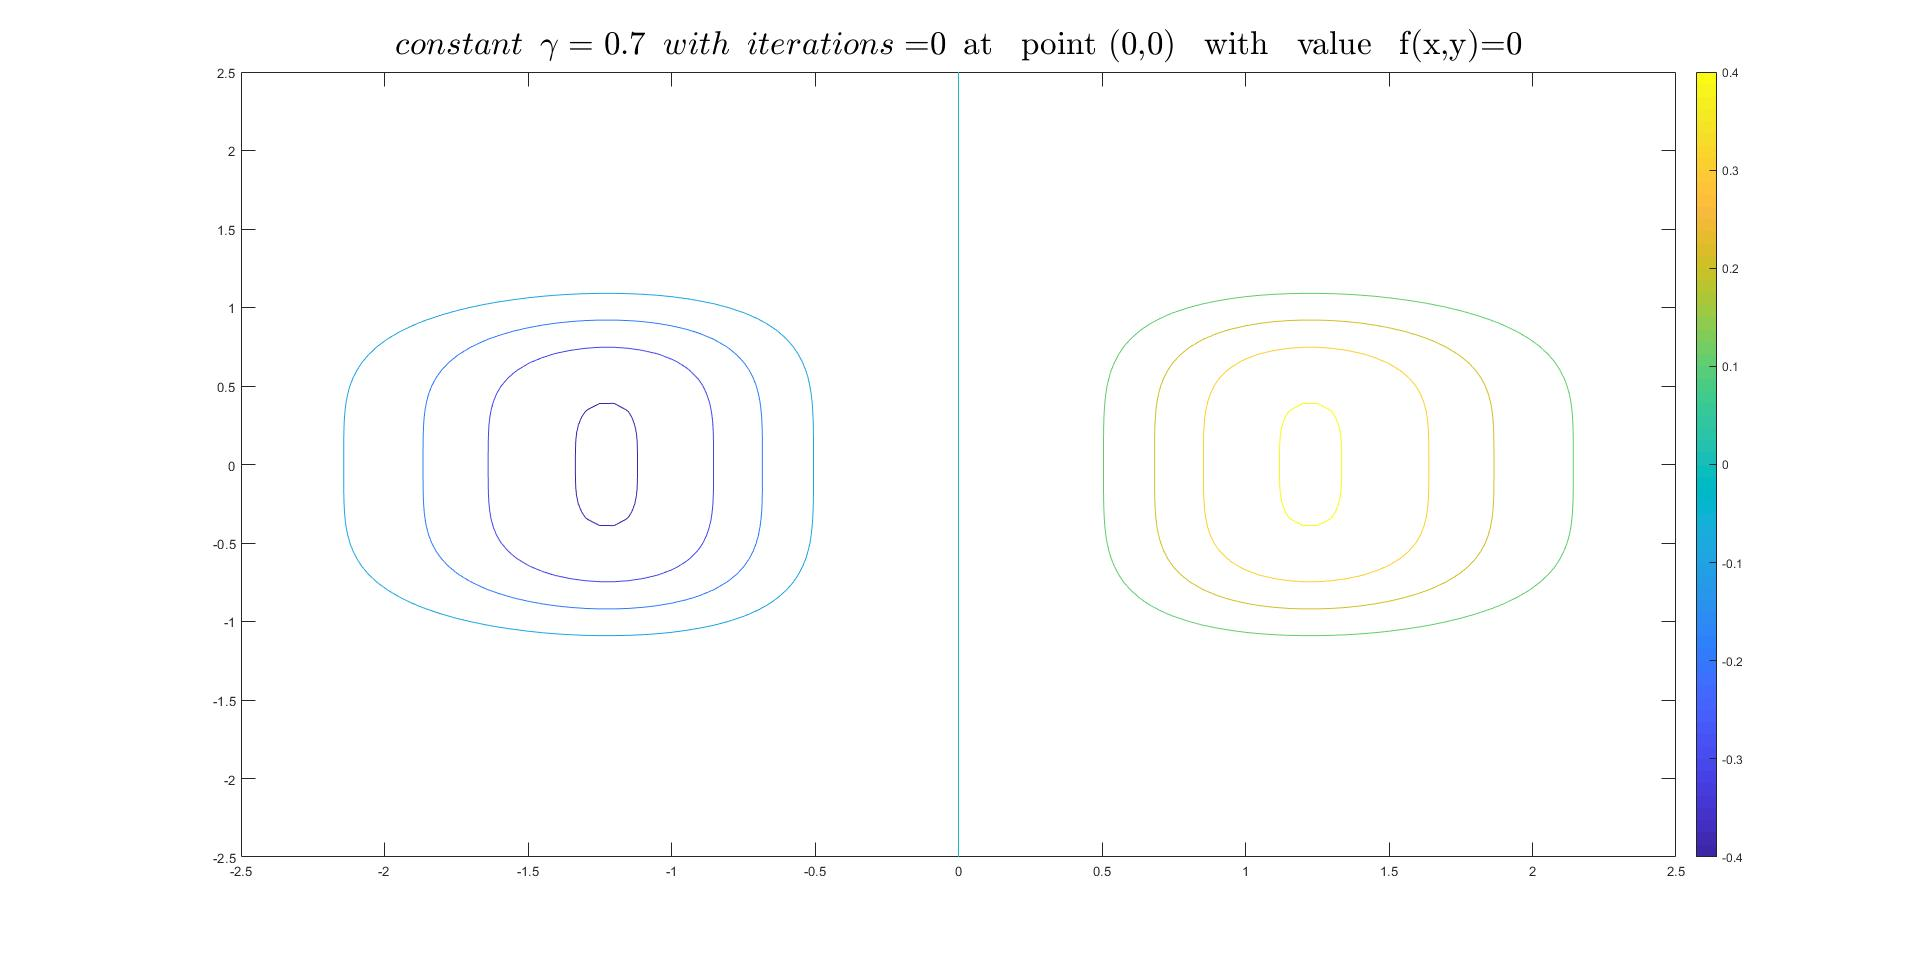
\includegraphics[width=140mm,scale=2]{n1aa.jpg}
\end{figure*} 
Για αρχικό σημείο (0,0) η παράγωγος της f είναι μηδέν οπότε ο αλγόριθμος τερματίζεται πρόωρα και συνεπώς εγκλωβιζόμαστε στο σημείο f(x,y)=0.
\subsubsection*{Αρχικό σημείο (-1,-1) για την συνάρτηση f}

Για αρχικό σημείο (-1,-1) ο αλγόριθμος τερματίζει αφού έχουμε αρνητικά ορισμένο εσσιανό πίνακα.
\clearpage
\subsubsection*{Αρχικό σημείο (1,1) για την συνάρτηση f}
 
Για αρχικό σημείο (1,1) ο αλγόριθμος τερματίζει αφού έχουμε αρνητικά ορισμένο εσσιανό πίνακα.
\subsubsection*{Αρχικό σημείο (-1,-0.5) για την συνάρτηση f}
\begin{figure*}[h!]	
     \centering  
     \advance\leftskip-0.2cm  
  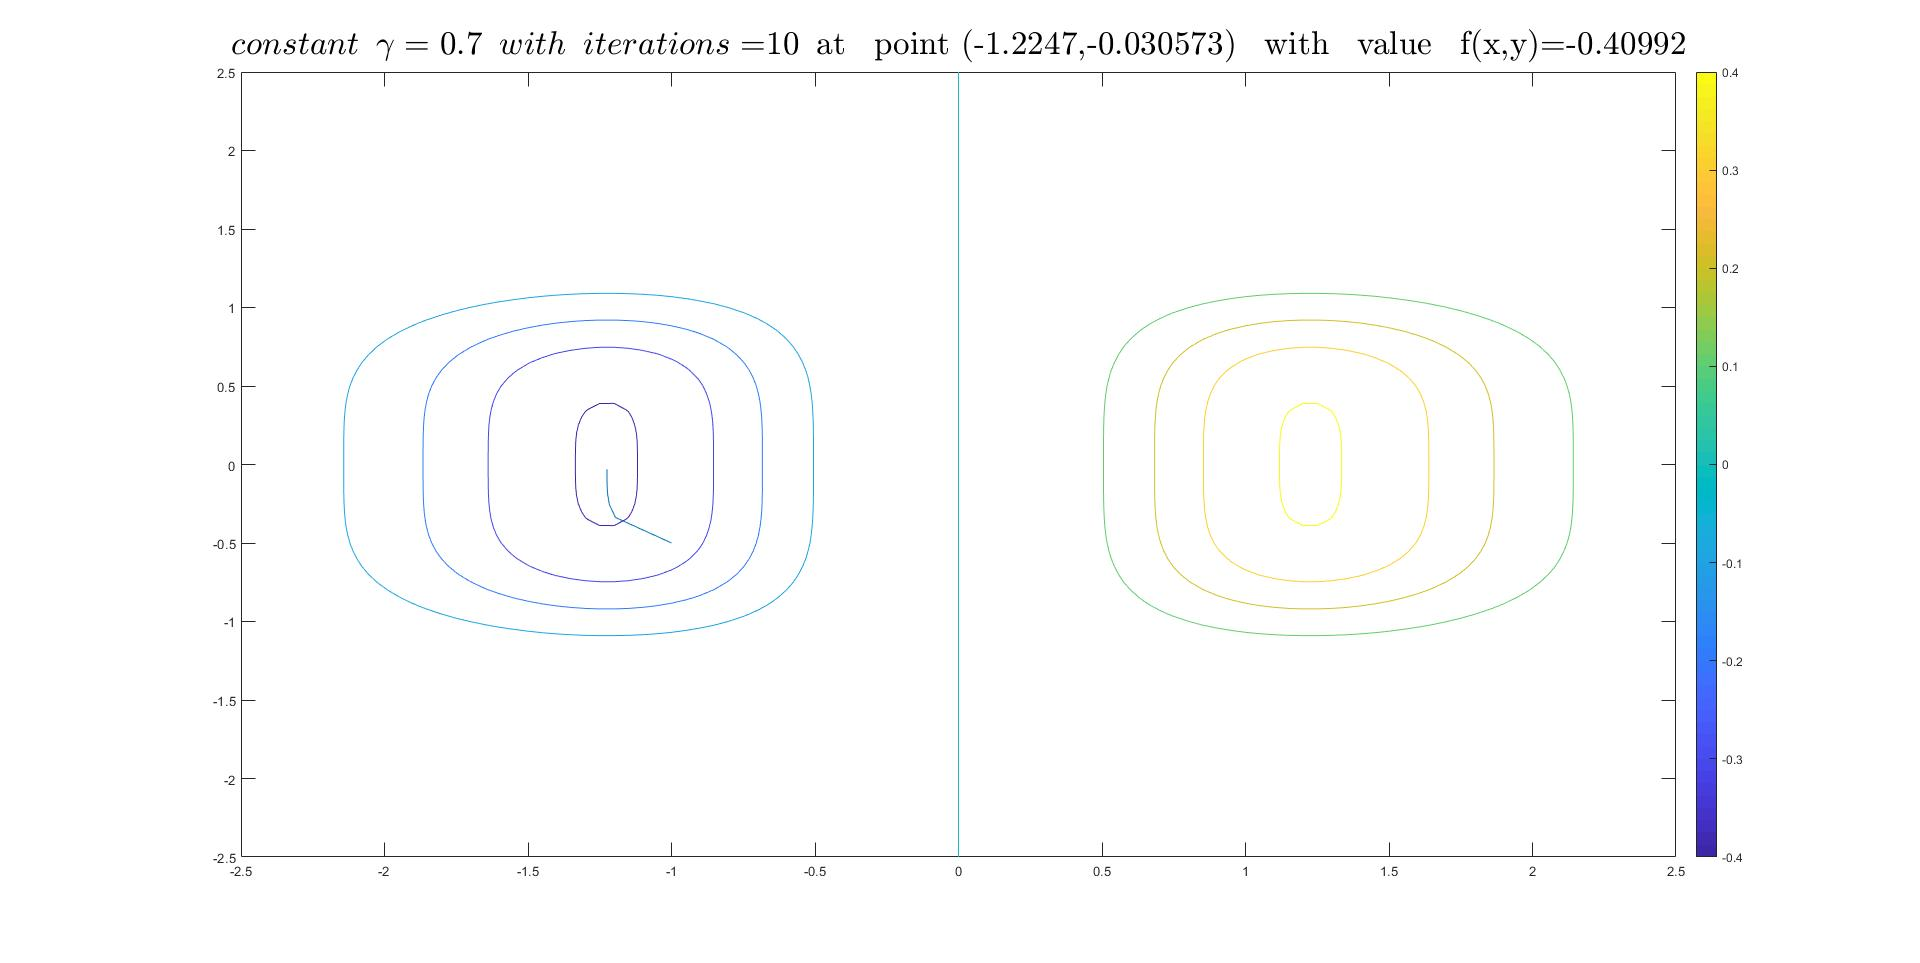
\includegraphics[width=140mm,scale=2]{n1a.jpg}
\end{figure*} 
Για αρχικό σημείο (-1,-0.5) μετά απο 10 επαναλήψεις καταλήγουμε στο σημείο (-1.22,-0.03) για  δοσμένη ακρίβεια e=$10^{-4}$ με τιμή f(x,y)=-0.409 που είναι  το \textbf{ολικό ελάχιστο}
\clearpage
\subsection*{Ελαχιστοποίηση $f(x_k+g_k \cdot d_k )$}
 
\subsubsection*{Αρχικό σημείο (0,0) για την συνάρτηση f}
\begin{figure*}[h!]	
     \centering  
     \advance\leftskip-0.2cm  
  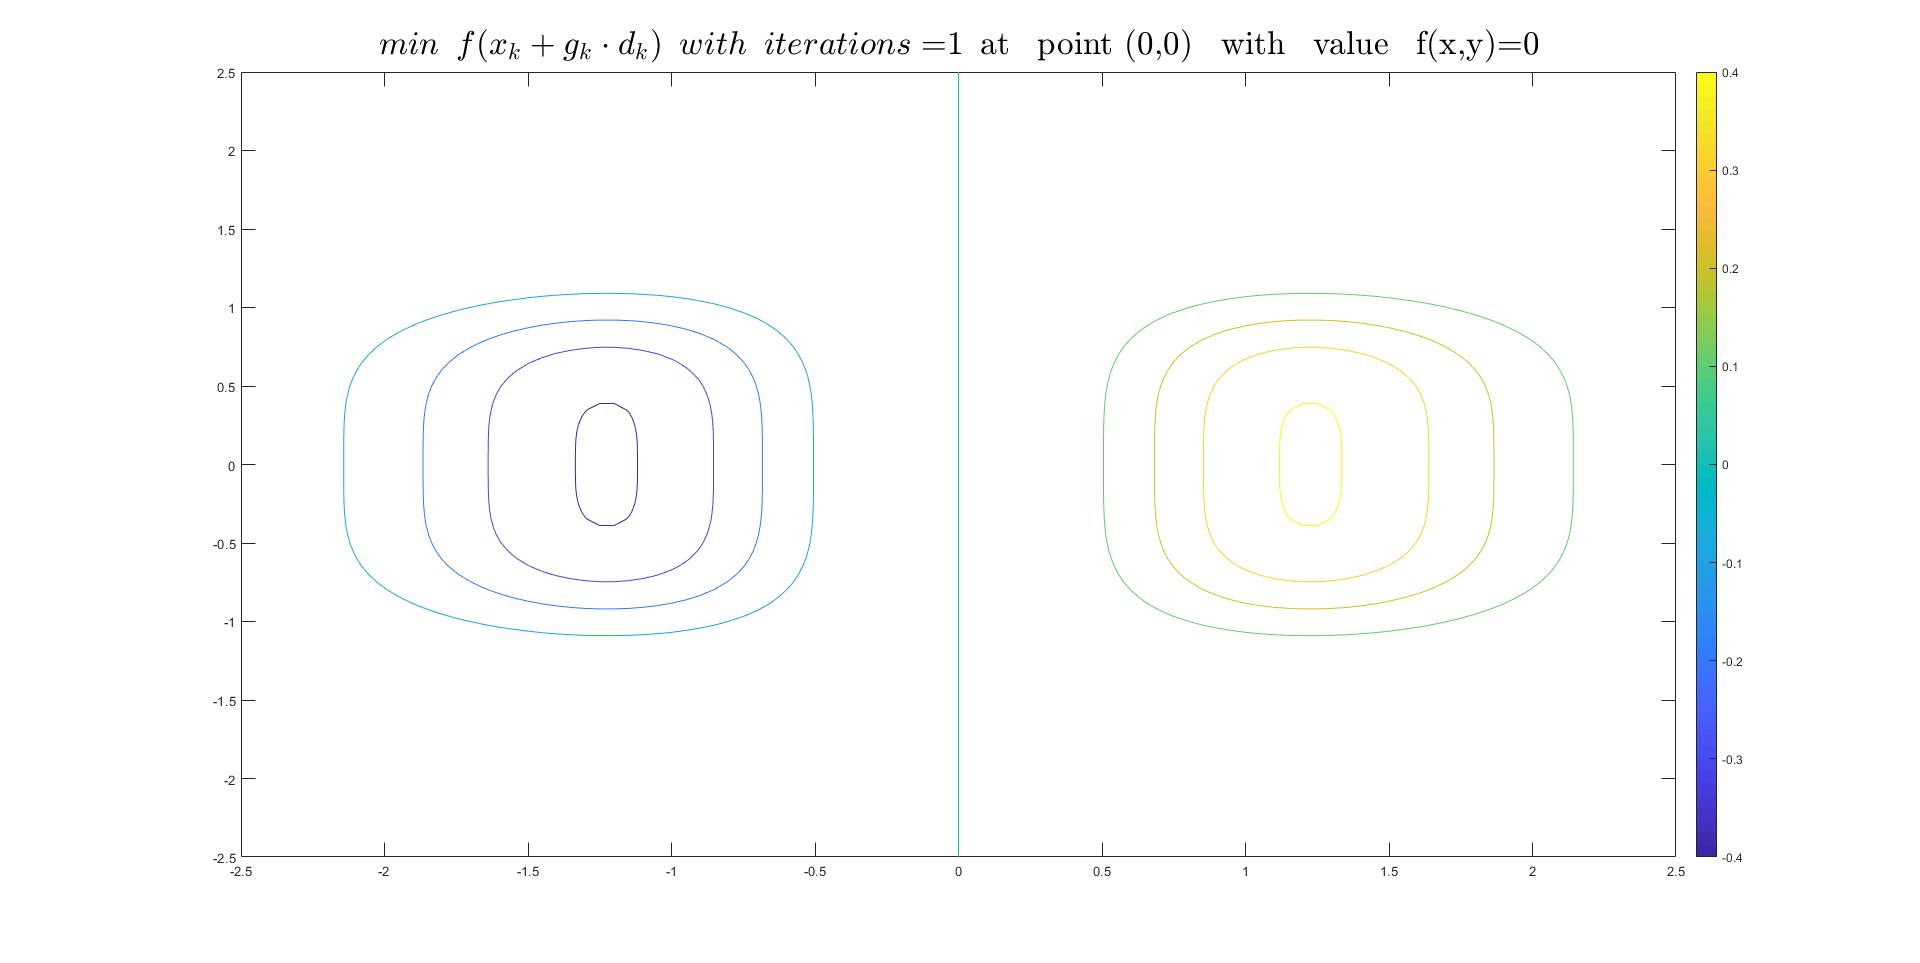
\includegraphics[width=140mm,scale=2]{mfa.jpg}
\end{figure*} 
Για αρχικό σημείο (0,0) η παράγωγος της f είναι μηδέν οπότε ο αλγόριθμος τερματίζεται πρόωρα και συνεπώς εγκλωβιζόμαστε στο σημείο f(x,y)=0.
 \subsubsection*{Αρχικό σημείο (-1,-1) για την συνάρτηση f}
Για αρχικό σημείο (-1,-1) ο αλγόριθμος τερματίζει αφού έχουμε αρνητικά ορισμένο εσσιανό πίνακα. 
 
\subsubsection*{Αρχικό σημείο (1,1) για την συνάρτηση f}
  
Για αρχικό σημείο (1,1) ο αλγόριθμος τερματίζει αφού έχουμε αρνητικά ορισμένο εσσιανό πίνακα. 
\clearpage
\subsubsection*{Αρχικό σημείο (-1,-0.5) για την συνάρτηση f}
\begin{figure*}[h!]	
     \centering  
     \advance\leftskip-0.2cm    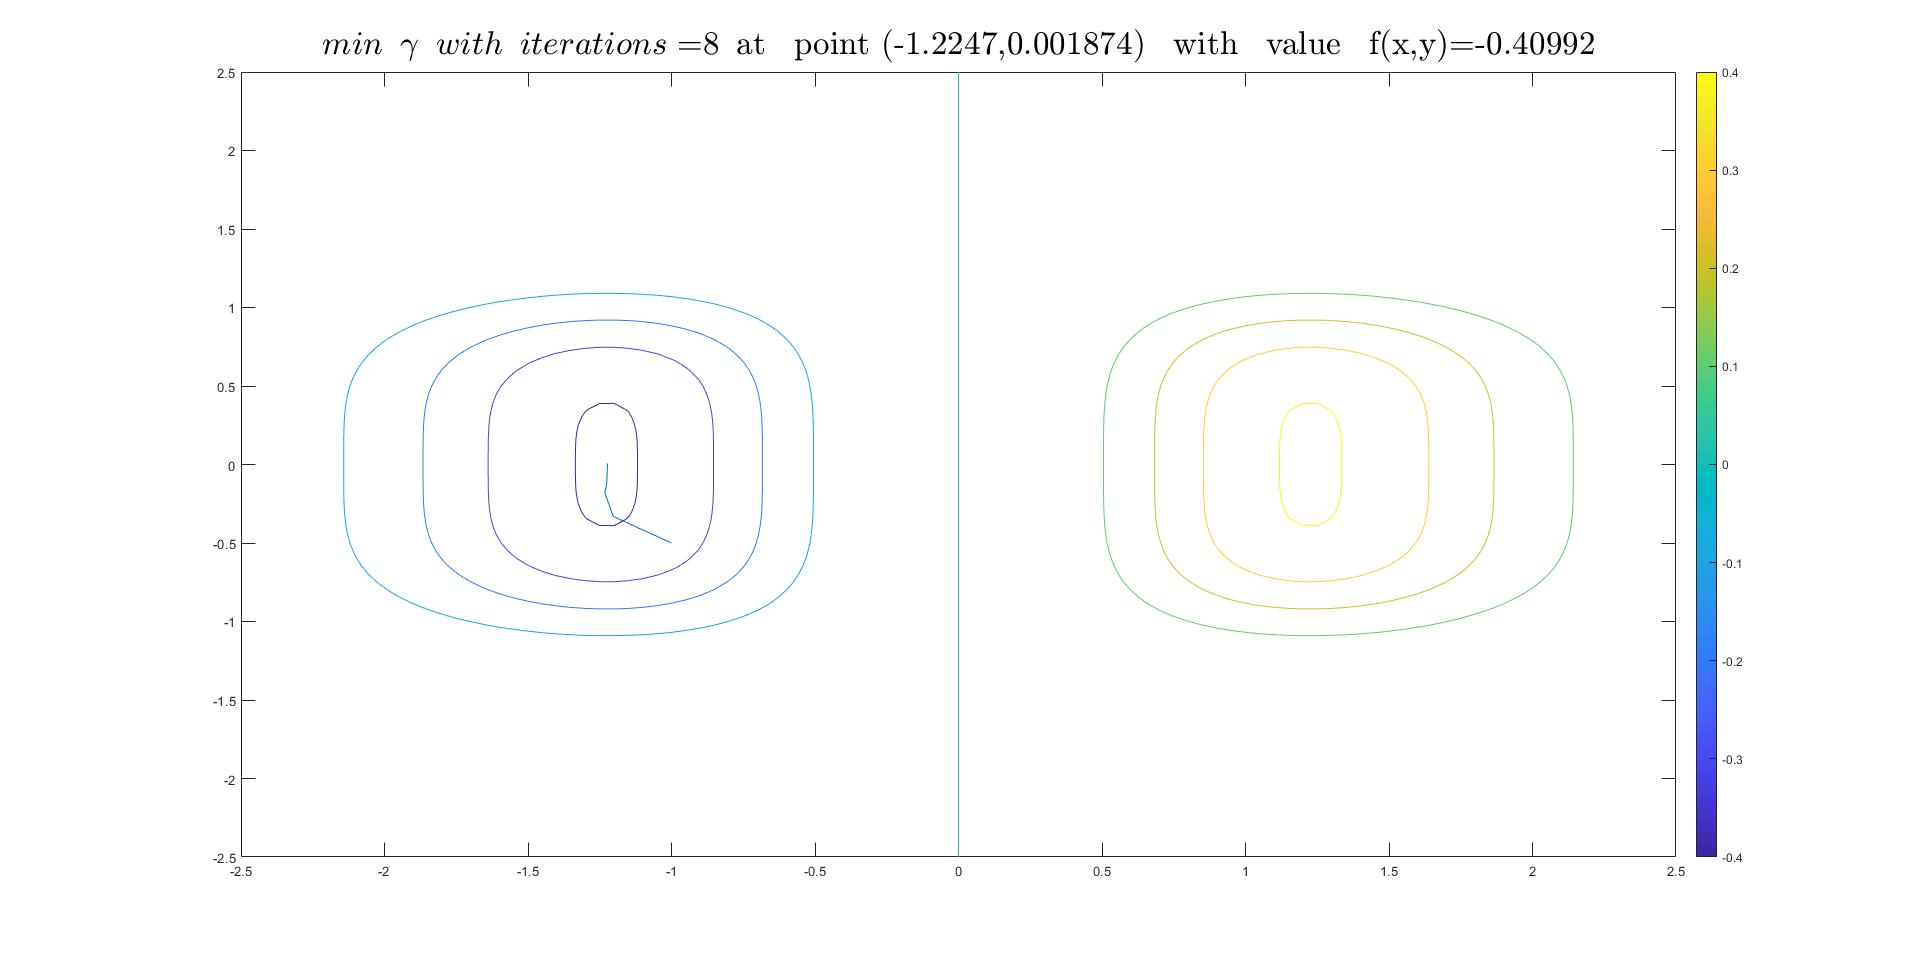
\includegraphics[width=140mm,scale=2]{mn2.jpg}
\end{figure*} 
Για αρχικό σημείο (-1,-0.5) μετά απο 8 επαναλήψεις καταλήγουμε στο σημείο (-1.22,-0.03) για  δοσμένη ακρίβεια e=$10^{-4}$ με τιμή f(x,y)=-0.409 που είναι  το \textbf{ολικό ελάχιστο} \clearpage
 \subsection*{Κανόνας Armijo}
\subsubsection*{Αρχικό σημείο (0,0) για την συνάρτηση f}
\begin{figure*}[h!]	
     \centering  
     \advance\leftskip-0.2cm  
  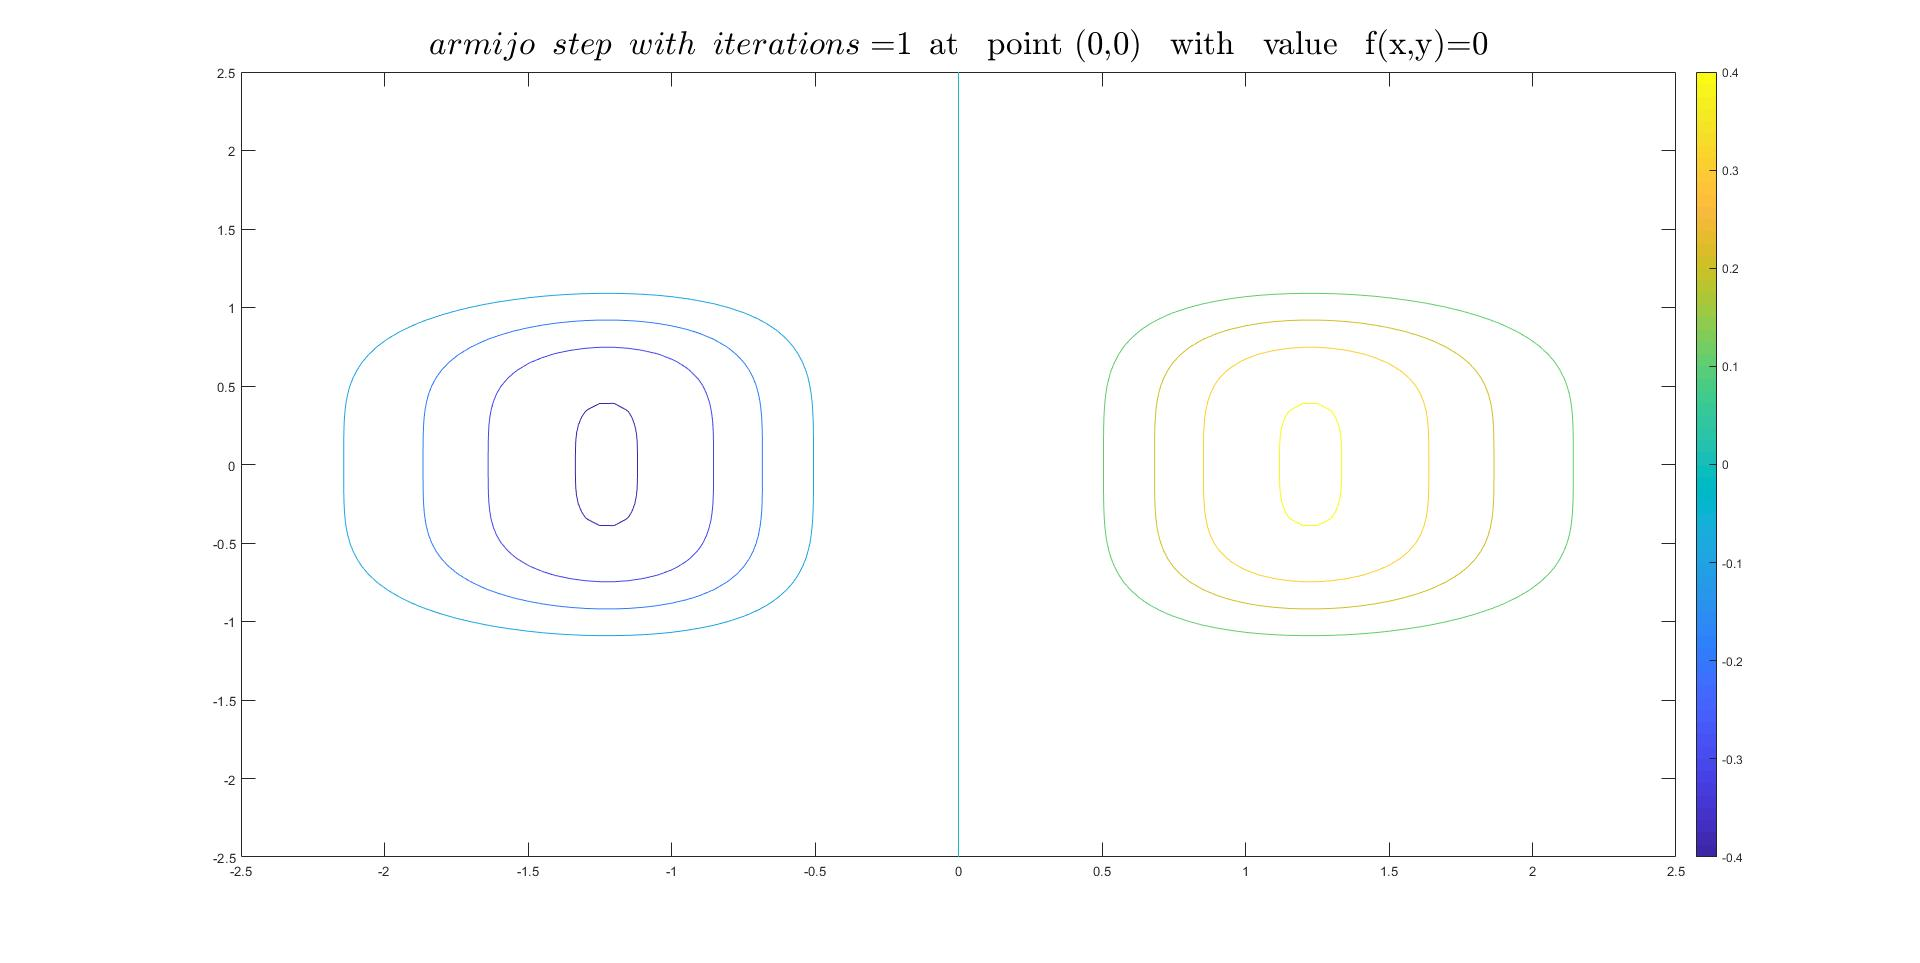
\includegraphics[width=130mm,scale=2]{arm1.jpg}
\end{figure*} 
Για αρχικό σημείο (0,0) η παράγωγος της f είναι μηδέν οπότε ο αλγόριθμος τερματίζεται πρόωρα και συνεπώς εγκλωβιζόμαστε στο σημείο f(x,y)=0.
\subsubsection*{Αρχικό σημείο (-1,-1) για την συνάρτηση f}
Για αρχικό σημείο (-1,-1) ο αλγόριθμος τερματίζει αφού έχουμε αρνητικά ορισμένο εσσιανό πίνακα. 
 
\subsubsection*{Αρχικό σημείο (1,1) για την συνάρτηση f}
  
Για αρχικό σημείο (1,1) ο αλγόριθμος τερματίζει αφού έχουμε αρνητικά ορισμένο εσσιανό πίνακα. 
\clearpage
\subsubsection*{Αρχικό σημείο (-1,-0.5) για την συνάρτηση f}
\begin{figure*}[h!]	
     \centering  
     \advance\leftskip-0.2cm    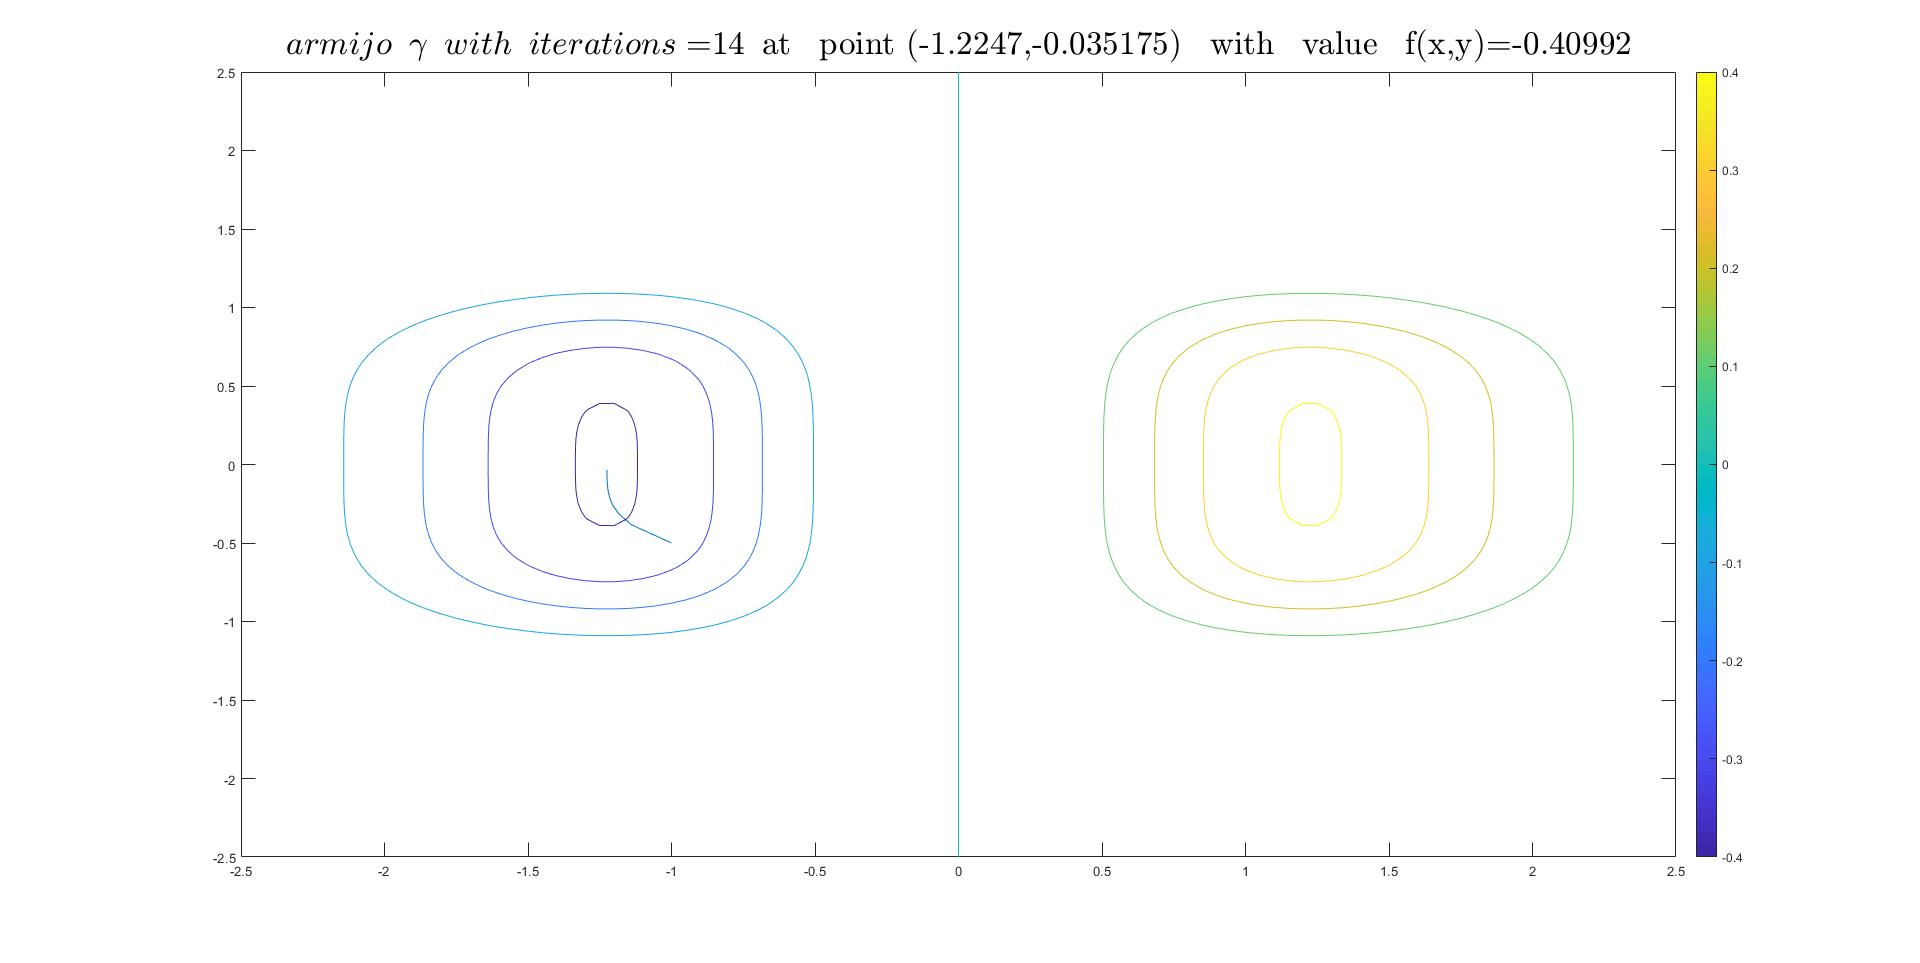
\includegraphics[width=140mm,scale=2]{armmin2.jpg}
\end{figure*} 
Για αρχικό σημείο (-1,-0.5) μετά απο 14 επαναλήψεις καταλήγουμε στο σημείο (-1.22,-0.03) για  δοσμένη ακρίβεια e=$10^{-4}$ με τιμή f(x,y)=-0.409 που είναι  το \textbf{ολικό ελάχιστο} \clearpage
\end{document}
